% Adapted directly from the official MJM bjourdoc.tex template.
\documentclass{birkjour}
%
% Do not add commands that alter page layout or fonts.
\usepackage[utf8]{inputenc}
\usepackage[T1]{fontenc}
\usepackage[english]{babel}
\usepackage{amsmath,amssymb,amsfonts,amsthm}
\usepackage{graphicx}
\usepackage{booktabs}
\usepackage{tabularx}
\usepackage{xcolor}
\usepackage{caption}
\usepackage{subcaption}
\usepackage{float}
\usepackage{url}
\usepackage{tikz}
\usetikzlibrary{arrows.meta,positioning}
\usepackage{hyperref}
\hypersetup{hidelinks}

% THEOREM environments follow bjourdoc.tex.
\newtheorem{theorem}{Theorem}[section]
\newtheorem{lemma}[theorem]{Lemma}
\newtheorem{proposition}[theorem]{Proposition}
\newtheorem{corollary}[theorem]{Corollary}
\theoremstyle{definition}
\newtheorem{definition}[theorem]{Definition}
\newtheorem{assumption}[theorem]{Assumption}
\theoremstyle{remark}
\newtheorem{remark}[theorem]{Remark}
\newtheorem*{ex}{Example}
\numberwithin{equation}{section}

\begin{document}

% Editorial commands: to be completed by the editorial office.
% \firstpage{1}
% \issuenumber{1}
% \Volumeandyear{...}
% \Copyrightyear{...}
% \DOI{...}
% \submitted{...}
% \received{...}
% \revised{...}
% \accepted{...}

% Insert title, affiliations and abstract as prescribed by bjourdoc.tex.
\title[Exact Partial-Sum Coercivity and Structure-Aware Benchmarks]
{Exact Partial-Sum Coercivity and \\
Structure-Aware Numerical Benchmarks \\
for Reaction--Diffusion Systems with Critical \\
Gradient Growth}

% The journal asks for a clear corresponding author and an active e-mail.
% Please add the verified e-mail(s) before submission; no address is invented here.
\author[Bouarifi]{Walid Bouarifi}
\address{Laboratory in Intelligent and Sustainable Technologies (LaRTID),\\
National School of Applied Sciences of Marrakech,\\
Cadi AYYAD University, Morocco}
\email{w.bouarifi@uca.ma}

\author[Alaa]{NourEddine Alaa}
\address{Faculty of Sciences and Techniques of Marrakech,\\
Cadi Ayyad University, Morocco}
\email{n.alaa@uca.ma}

\subjclass{Primary 35K57, 35D30; Secondary 65M60, 68T07}

\keywords{Reaction--diffusion systems, critical gradient growth, partial-sum estimate, energy identity, physics-informed neural networks, finite elements}

\begin{abstract}
We derive the exact partial-sum energy identity underlying weak-solution arguments for triangular reaction--diffusion systems with critical gradient growth. The exact cross terms involve the full gradients of preceding components; when these gradients are independently bounded in $L^2(Q_T)$, a free Young parameter absorbs all cross terms for any fixed positive diffusion vector, without an ordering restriction at this conditional coercivity step. The analytical statement is deliberately separated from the additional compactness ingredients required for a global-existence theorem. Numerically, we first verify the classical solvers with a forced manufactured solution. Independent spatial refinement gives observed RMSE orders between $1.98$ and $2.00$ for the semi-implicit finite-difference method and the assembled $P_1$ Galerkin method, while temporal refinement gives first-order behaviour. We then retain the two-component PINN--FDM--FEM comparison: FEM and FDM attain RMSE values $8.87\times10^{-5}$ and $1.32\times10^{-4}$ against a refined reference, whereas the nonnegative boundary-compatible PINN attains $(3.37\pm0.54)\times10^{-3}$ over five seeds, with a relative initial-data mismatch of $4.24\%\pm0.38\%$. Finally, a three-component benchmark with the non-monotone diffusion vector $(0.1,0.8,0.3)$ realizes the simultaneous cross-term setting. The required preceding-gradient bounds are obtained directly from component energy identities, giving $C_1\le1.2$, $C_2\le0.07090$, and a residual Young contribution bounded by $0.32136$. These experiments provide structure-aware diagnostics for the analytical estimate while separating PINN field error, initial-data mismatch, and residual generalization on the tested forward problem.
\end{abstract}

\maketitle

% -----------------------------------------------------------------------------
% Main text
% -----------------------------------------------------------------------------
\section{Introduction}
\label{sec:introduction}

Reaction--diffusion systems with gradient-dependent nonlinearities arise when local production, dissipation, or transfer mechanisms depend on spatial variations of the state. We consider
\begin{equation}
\begin{cases}
\partial_tu_i-d_i\Delta u_i=f_i(t,x,u,\nabla u), &(t,x)\in Q_T=(0,T)\times\Omega,\\
u_i(0,x)=u_{i,0}(x),&x\in\Omega,\\
u_i(t,x)=0,&(t,x)\in(0,T)\times\partial\Omega,
\end{cases}
\qquad i=1,\ldots,m,
\label{eq:main_system}
\end{equation}
where $\Omega\subset\mathbb R^N$ is bounded and $d_i>0$. Quadratic dependence on $\nabla u$ is critical for the compactness and equi-integrability arguments used to construct weak solutions. At the modelling level, such terms describe rates that become stronger near steep spatial fronts and can therefore serve as reduced representations of interfacial transfer, gradient-enhanced dissipation, or front-localized conversion. The present work studies a mathematically representative prototype; application-specific constitutive validity would require dimensional derivation, parameter calibration, and observational validation.

\subsection{Related work and research gap}
\label{subsec:related-work}

\paragraph{Analytical background.}
Global existence and boundedness for reaction--diffusion systems under mass control or mass dissipation have been developed through several complementary mechanisms. Classical results established global existence under structural assumptions linking reaction terms and diffusion~\cite{hollis1987global,boudiba2000coupled}, while later work clarified the role of mass control, quadratic growth, duality, and intermediate-sum structures~\cite{pierre2010survey,souplet2018quadratic,fellner2020quadratic,cupps2021uniform,morgan2020intermediate}. Critical natural growth with respect to the gradient is substantially more delicate because weak compactness of the state variables alone does not automatically control nonlinear expressions involving $|\nabla u|^2$. Scalar critical-gradient problems were treated by Landes and Mustonen~\cite{landes1994parabolic}; for systems, Alaa and Mounir considered a two-component critical-gradient setting~\cite{alaa2001global}, and triangular $m$-component extensions with low-regularity data were subsequently developed in~\cite{alaa2013triangular,bouarifi2015climate}.

The published scope of the two triangular references is important for positioning the present result accurately. Reference~\cite{alaa2013triangular} establishes weak-solution existence for $m\times m$ triangular systems with nonnegative solutions, $L^1$ data, and critical gradient growth, whereas~\cite{bouarifi2015climate} develops a related critical-gradient triangular existence framework in an energy-balance climate setting. Those references provide the theorem-level context. Here we isolate one local coercivity step, re-derive it from the regularized equations, and state exactly which full-gradient information that step requires. The resulting contribution is specific: the exact cross-gradient identity, the exposed full-gradient hypothesis, and the conditional removal of diffusion ordering at the absorption stage.

The analytical gap is a precise one inside the existing global-existence framework. When the first $r$ regularized equations are summed and tested by $T_k(U_{r,n})$, direct integration by parts produces cross terms containing the \emph{full} gradients $\nabla u_{j,n}$ of preceding components. Replacing them by $\nabla T_k(u_{j,n})$ changes the localization set and therefore changes the estimate being proved. The resulting question is precise: once full $L^2(Q_T)$ bounds for the preceding gradients are independently available, is an ordering of the positive diffusion coefficients still needed to absorb the cross terms? We show that it is not: conditional on the independently available full-gradient bounds, a free Young parameter absorbs all such terms for any fixed positive diffusion vector. The novelty does not lie in Young's inequality itself. It lies in identifying the exact cross-gradient structure generated by the partial-sum test, isolating the full-gradient hypothesis that is genuinely required, and showing that once this hypothesis is available no monotone ordering of the diffusion coefficients is needed at the coercivity stage. The contribution is therefore the exact identity together with this conditional coercivity clarification and an explicit separation from the additional compactness, equi-integrability, and nonlinear limit-identification arguments required for existence.

\paragraph{Numerical verification and classical discretizations.}
Because the analytical claim is paired with numerical evidence, implementation verification must be separated from comparison against a refined numerical reference. For parabolic problems, standard Galerkin theory and time-discretization analysis provide the classical context for $P_1$ finite elements and implicit--explicit reaction--diffusion updates~\cite{thomee2006galerkin,hundsdorfer2003adr}. We therefore use the Method of Manufactured Solutions (MMS), a standard code-verification methodology in which a smooth analytical field is prescribed and the corresponding forcing terms are obtained by substitution into the governing equations~\cite{roache2002mms,oberkampf2010vv}. Separate spatial and temporal refinements then test whether the implemented FDM and FEM recover their expected asymptotic behavior, independently of the unforced reference computation used later for method comparison.

\paragraph{Physics-informed neural networks.}
Physics-informed neural networks (PINNs) embed differential-equation residuals and data constraints into the training objective~\cite{raissi2019physics}; software frameworks and broader scientific-machine-learning surveys have accelerated their use for forward and inverse differential problems~\cite{lu2021deepxde,cuomo2022sciml}. Their flexibility, however, does not make optimization or error control automatic. Training can suffer from severe loss-gradient imbalance and unequal convergence of objective components~\cite{wang2021gradient}, neural-tangent-kernel analyses reveal mechanisms behind training failure~\cite{wang2022ntk}, and empirical studies show that a small training loss may coexist with a substantial solution error~\cite{krishnapriyan2021failure}. Rigorous analyses available for selected PDE classes likewise distinguish training, generalization, and field errors and require stability, regularity, and sampling assumptions to connect them~\cite{deryck2022error,mishra2023generalization,deryck2024numerical}. For time-dependent PDEs, causality-aware strategies can improve training~\cite{wang2024causality}, while residual-based adaptive sampling has been shown to materially affect accuracy and sampling efficiency~\cite{wu2023sampling}. Exact imposition of Dirichlet conditions through the network output is also an active design choice rather than a cosmetic one~\cite{berrone2023dirichlet}.

These observations define the computational research gap of the present paper. A credible comparison should not use a PINN training loss as its only validation quantity, nor should it compare an unverified classical implementation against a learned surrogate. We therefore combine: (i) independent MMS verification of FDM and FEM; (ii) a common refined-reference comparison for PINN, FDM, and FEM; (iii) a common-point residual test excluded from PINN training; (iv) positivity, partial-mass, and energy diagnostics; and (v) a three-component non-monotone benchmark that directly exercises the multiple cross terms occurring in the analytical estimate.

\subsection{Contributions and scientific architecture}

The contributions are:
\begin{enumerate}
 \item the exact partial-sum identity and a parametric Young estimate valid for any fixed positive diffusion vector under explicit preceding-gradient bounds;
 \item an explicit statement of the logical dependence between the exact estimate and the compactness theory developed in earlier work;
 \item an independent manufactured-solution verification showing approximately second-order spatial and first-order temporal behaviour for the classical discretizations;
 \item a reproducible two-component PINN--FDM--FEM diagnostic comparison with five-seed variability, independent residual testing, explicit initial-data error, refinement checks, mass and energy diagnostics, and a collocation-size ablation;
 \item a three-component non-monotone benchmark with two simultaneous cross terms and energy-derived preceding-gradient bounds;
 \item a constraint-compatible PINN representation that enforces non-negativity and homogeneous Dirichlet values exactly while leaving the initial condition penalized and quantitatively auditable.
\end{enumerate}

\begin{figure}[H]
\centering
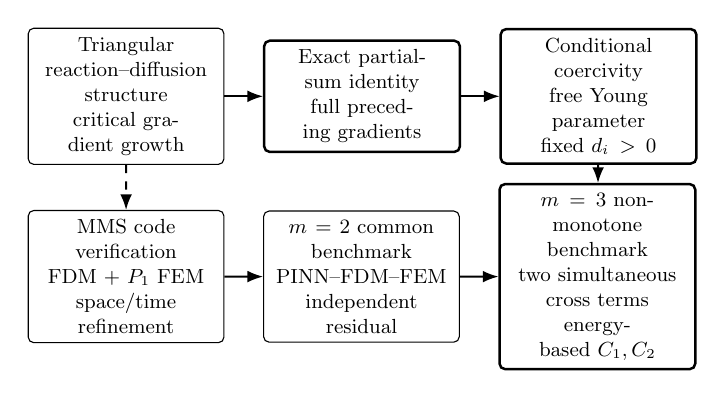
\begin{tikzpicture}[
  scale=.82,
  transform shape,
  node distance=7mm and 6mm,
  box/.style={draw, rounded corners=2pt, align=center, minimum height=10mm, text width=2.75cm, inner sep=4pt, font=\small},
  emph/.style={box, line width=0.9pt},
  arrow/.style={-{Latex[length=2mm]}, line width=0.7pt},
  dashedarrow/.style={-{Latex[length=2mm]}, dashed, line width=0.7pt}
]
\node[box] (structure) {Triangular reaction--diffusion structure\\critical gradient growth};
\node[emph, right=of structure] (identity) {Exact partial-sum identity\\full preceding gradients};
\node[emph, right=of identity] (coercivity) {Conditional coercivity\\free Young parameter\\fixed $d_i>0$};

\node[box, below=of structure] (mms) {MMS code verification\\FDM + $P_1$ FEM\\space/time refinement};
\node[box, right=of mms] (two) {$m=2$ common benchmark\\PINN--FDM--FEM\\independent residual};
\node[emph, right=of two] (three) {$m=3$ non-monotone benchmark\\two simultaneous cross terms\\energy-based $C_1,C_2$};

\draw[arrow] (structure) -- (identity);
\draw[arrow] (identity) -- (coercivity);
\draw[arrow] (mms) -- (two);
\draw[arrow] (two) -- (three);
\draw[dashedarrow] (coercivity) -- (three);
\draw[dashedarrow] (structure) -- (mms);
\end{tikzpicture}
\caption{Scientific architecture of the paper.}
\label{fig:scientific-architecture}
\end{figure}

Figure~\ref{fig:scientific-architecture} summarizes the logic of the paper. The upper path represents analytical implication, whereas the lower path represents numerical verification and diagnostic comparison. The two paths are deliberately kept logically distinct and meet only at the level of a controlled numerical illustration: the three-component benchmark realizes the non-monotone diffusion configuration and independently available preceding-gradient estimates without being used as a proof of the analytical proposition.

Section~\ref{sec:theoretical} gives the analytical derivation. Section~\ref{sec:numerical} presents the common numerical protocol, Section~\ref{sec:results} reports the computed results and ablations, and Section~\ref{sec:conclusion} concludes.

\section{Analytical framework and exact partial-sum estimate}
\label{sec:theoretical}

The two-component critical case was treated in~\cite{alaa2001global}, and complete triangular $m$-component existence frameworks were developed in~\cite{alaa2013triangular,bouarifi2015climate}. The present section isolates a narrower analytical object inside that setting: the exact partial-sum coercivity calculation and the full-gradient hypothesis it actually uses. Conditional on those bounds, the absorption step is valid for any fixed positive diffusion vector without monotone ordering.

\subsection{Assumptions and solution concept}

Let $T_k(s)=\max(-k,\min(s,k))$. We assume that $\Omega\subset\mathbb R^N$ is bounded with Lipschitz boundary, $d_i>0$, and $u_{i,0}\in L^2(\Omega)$ is nonnegative. The nonlinearities are Carathéodory functions, locally Lipschitz in $(u,p)$, and quasi-positive:
\[
 f_i(t,x,u_1,\ldots,u_{i-1},0,u_{i+1},\ldots,u_m,p_1,\ldots,p_{i-1},0,p_{i+1},\ldots,p_m)\ge0
\]
for $u\in\mathbb R_+^m$. We use the partial-sum form of triangular control
\begin{equation}
 \sum_{i=1}^r f_i(t,x,u,p)\le0,
 \qquad r=1,\ldots,m,
 \label{eq:partial-mass}
\end{equation}
which is a special case of the standard weighted lower-triangular condition. The critical-growth assumptions are
\begin{align}
 |f_1(t,x,u,p)|&\le \Gamma_1(|u_1|)\left(F_1+|p_1|^2+\sum_{j=2}^m|p_j|^{\alpha_j}\right),\quad 1\le\alpha_j<2,\label{eq:growth1}\\
 |f_i(t,x,u,p)|&\le \Gamma_i\left(\sum_{j=1}^i|u_j|\right)\left(F_i+\sum_{j=1}^m|p_j|^2\right),\quad i\ge2,\label{eq:growth2}
\end{align}
where $F_i\in L^1(Q_T)$ and the $\Gamma_i$ are nondecreasing. This notation is kept distinct from the constants $C_j$ introduced below for full-gradient bounds.
The growth assumptions identify the critical framework in which the partial-sum calculation is used. They are not needed for the algebraic identity or for Young's inequality itself; their role belongs to the separate estimates, equi-integrability, and limit passage required by a complete existence proof. This distinction is essential to the scope of Proposition~\ref{prop:partial-sum}.

A vector $u=(u_1,\ldots,u_m)$ is a weak solution on $Q_T$ if
\[
 u_i\in C([0,T];L^1(\Omega))\cap L^2(0,T;H_0^1(\Omega)),\qquad
 f_i(\cdot,u,\nabla u)\in L^1(Q_T),
\]
and, for every $\varphi\in C_c^\infty([0,T)\times\Omega)$,
\[
 -\int_{Q_T}u_i\partial_t\varphi+d_i\int_{Q_T}\nabla u_i\cdot\nabla\varphi
 =\int_\Omega u_{i,0}\varphi(0,\cdot)+\int_{Q_T}f_i(t,x,u,\nabla u)\varphi.
\]
This weak formulation is the only solution concept used below.

\subsection{Approximation scheme}

For completeness, let $u_{i,0}^n\in C_c^\infty(\Omega)$ be nonnegative approximations converging to $u_{i,0}$ in $L^2(\Omega)$. Let $\chi_n$ be a smooth cut-off equal to one on $[0,n]$ and zero on $[2n,\infty)$, and define
\[
 f_i^n(t,x,u,p)=\chi_n(|u|+|p|)f_i(t,x,u,p).
\]
Because the same nonnegative scalar cut-off multiplies every component, the partial-sum sign is preserved pointwise:
\[
 \sum_{i=1}^r f_i^n=\chi_n(|u|+|p|)\sum_{i=1}^r f_i\le0.
\]
Using component-dependent cut-offs would not provide this implication and would require a separate argument.

The same common cut-off also preserves quasi-positivity: since $\chi_n\ge0$, each $f_i^n$ has the same nonnegative boundary-face sign as $f_i$. For the sufficiently regular approximants used below, the standard invariant-region (equivalently, first-contact/negative-part) argument therefore preserves the nonnegative cone from nonnegative initial data and homogeneous Dirichlet boundary values. Hence
\[
u_{i,n}\ge0,\qquad U_{r,n}=\sum_{j=1}^r u_{j,n}\ge0,\qquad T_k(U_{r,n})\ge0.
\]
Combining this with $\sum_{j=1}^r f_j^n\le0$ yields the signed reaction estimate
\[
\left(\sum_{j=1}^r f_j^n\right)T_k(U_{r,n})\le0,
\]
which is the implication used in Proposition~\ref{prop:partial-sum}.

The regularized problem is
\begin{equation}
 \partial_tu_{i,n}-d_i\Delta u_{i,n}=f_i^n(t,x,u_n,\nabla u_n),
 \quad u_{i,n}|_{\partial\Omega}=0,
 \quad u_{i,n}(0)=u_{i,0}^n.
 \label{eq:approx-system}
\end{equation}
For the energy calculation, we work with sufficiently regular nonnegative solutions of~\eqref{eq:approx-system}; such regularity may be obtained through an additional smoothing of the data and nonlinearities in the standard approximation procedure. The algebra below is independent of the particular smoothing. We write
\[
 U_{r,n}=\sum_{j=1}^r u_{j,n}.
\]

\subsection{Exact partial-sum energy identity and parametric absorption}

Define the primitive
\[
 \Phi_k(s)=\int_0^sT_k(\tau)\,d\tau.
\]
It is nonnegative, satisfies $0\le\Phi_k(s)\le k|s|$, and obeys the Sobolev chain rules
\[
 \partial_t\Phi_k(U_{r,n})=T_k(U_{r,n})\partial_tU_{r,n},\qquad
 \nabla T_k(U_{r,n})=\mathbf 1_{\{|U_{r,n}|<k\}}\nabla U_{r,n}
\]
almost everywhere (with the usual regularized interpretation at the two truncation levels). These facts justify the time term and the principal diffusion term below.
Summing the first $r$ equations of~\eqref{eq:approx-system}, with $U_{r,n}=\sum_{j=1}^r u_{j,n}$, gives the exact differential identity
\begin{equation}
 \partial_tU_{r,n}-d_r\Delta U_{r,n}
 =\sum_{j=1}^r f_j^n
  +\sum_{j=1}^{r-1}(d_j-d_r)\Delta u_{j,n}.
 \label{eq:exact-sum-equation}
\end{equation}
Testing~\eqref{eq:exact-sum-equation} by $T_k(U_{r,n})$, integrating over $(0,t)\times\Omega$, and using the homogeneous Dirichlet conditions yields
\begin{align}
 &\int_\Omega\Phi_k(U_{r,n}(t))
 +d_r\int_0^t\!\!\int_\Omega|\nabla T_k(U_{r,n})|^2 \nonumber\\
 &\quad=\int_\Omega\Phi_k(U_{r,n}(0))
 +\int_0^t\!\!\int_\Omega\left(\sum_{j=1}^rf_j^n\right)T_k(U_{r,n}) \nonumber\\
 &\qquad\quad+\sum_{j=1}^{r-1}(d_r-d_j)
 \int_0^t\!\!\int_\Omega\nabla u_{j,n}\cdot\nabla T_k(U_{r,n}).
 \label{eq:exact-partial-energy}
\end{align}
Equation~\eqref{eq:exact-partial-energy}, rather than an identity involving $\nabla T_k(u_{j,n})$, is the direct consequence of the approximating equations. Indeed,
\[
 \nabla T_k(u_{j,n})=\mathbf 1_{\{|u_{j,n}|<k\}}\nabla u_{j,n},\qquad
 \nabla T_k(U_{r,n})=\mathbf 1_{\{|U_{r,n}|<k\}}\sum_{\ell=1}^r\nabla u_{\ell,n}.
\]
The two indicator sets are generally different. Hence multiplication by $\nabla T_k(U_{r,n})$ does not localize $\nabla u_{j,n}$ to $\{|u_{j,n}|<k\}$, and replacing the former by $\nabla T_k(u_{j,n})$ would change the identity. This observation is the precise reason why full, rather than merely truncated, preceding-gradient control appears in Lemma~\ref{lem:parametric-young}.

\begin{assumption}[Preceding-gradient bound]\label{ass:previous-full-gradient}
Let $r\ge2$ and $d_1,\ldots,d_r>0$. For $j=1,\ldots,r-1$, assume
\begin{equation}
 \sup_n\int_{Q_T}|\nabla u_{j,n}|^2\le C_j.
 \label{eq:previous-full-gradient}
\end{equation}
\end{assumption}

\begin{lemma}[Parametric control of the exact cross terms]
\label{lem:parametric-young}
Under Assumption~\ref{ass:previous-full-gradient}, the cross terms in~\eqref{eq:exact-partial-energy} can be absorbed into the principal $U_{r,n}$ term without ordering the diffusion coefficients.
\end{lemma}

\begin{proof}
Put $a_j=|d_r-d_j|$ and $A_r=\sum_{j<r}a_j$. For every $\varepsilon>0$,
\[
 (d_r-d_j)\nabla u_{j,n}\cdot\nabla T_k(U_{r,n})
 \le \frac{\varepsilon a_j}{2}|\nabla T_k(U_{r,n})|^2
 +\frac{a_j}{2\varepsilon}|\nabla u_{j,n}|^2.
\]
If $A_r=0$, all cross terms vanish. Otherwise choose $\varepsilon=d_r/A_r$. Summation leaves at least $d_r/2$ of the principal diffusion term on the left and bounds the remaining contribution by
\[
 \sum_{j<r}\frac{a_jA_r}{2d_r}C_j.
\]
The constants depend on the fixed diffusion vector but not on $n$. Since $u_{i,0}^n\to u_{i,0}$ in $L^2(\Omega)$, the initial terms are also uniformly bounded for every fixed $k$.
\end{proof}

\begin{proposition}[Exact partial-sum estimate]
\label{prop:partial-sum}
Assume the regularized solutions are nonnegative, the common cut-off preserves the partial-sum sign $\sum_{j=1}^r f_j^n\le0$, and Assumption~\ref{ass:previous-full-gradient} holds. Then $T_k(U_{r,n})\ge0$, so the reaction contribution in~\eqref{eq:exact-partial-energy} is nonpositive. For every $t\le T$,
\[
 \frac{d_r}{2}\int_0^t\!\!\int_\Omega|\nabla T_k(U_{r,n})|^2
 \le \int_\Omega\Phi_k(U_{r,n}(0))
 +\sum_{j<r}\frac{a_jA_r}{2d_r}C_j,
\]
uniformly in $n$. No monotone ordering of the fixed positive vector $(d_1,\ldots,d_r)$ is required at this absorption step.
\end{proposition}

\begin{proof}
Use the sign of the reaction term in~\eqref{eq:exact-partial-energy}, discard the nonnegative terminal term $\int_\Omega\Phi_k(U_{r,n}(t))$, and apply Lemma~\ref{lem:parametric-young}.
\end{proof}

\begin{remark}
The estimate is conditional on full $L^2$ gradient bounds for the preceding components. Bounds only for $\nabla T_k(u_{j,n})$ do not control the exact cross terms in~\eqref{eq:exact-partial-energy}. Consequently, the estimate applies within frameworks in which Assumption~\ref{ass:previous-full-gradient}, equivalently~\eqref{eq:previous-full-gradient}, has already been established. The value of Proposition~\ref{prop:partial-sum} is therefore not to generate the preceding-gradient estimates, but to separate their derivation from the subsequent partial-sum coercivity step. Any independently available componentwise energy, entropy, or duality estimate may be inserted at this point; once the full-gradient bounds are available, no monotone ordering of the diffusion coefficients is needed for the absorption step. This hypothesis should be stated whenever the proposition is used.
\end{remark}
\subsection{Relation to the earlier triangular arguments}

For the historical formulations and the complete compactness constructions, the reader is referred to the partial-sum arguments developed for critical-gradient triangular systems in~\cite{alaa2013triangular,bouarifi2015climate}. Rather than relying on equation numbers that may vary between published and archived versions, we reproduce here the relevant calculation in a self-contained form. When the coefficients $d_j$ differ, direct integration by parts yields the cross-diffusion contribution $\nabla u_{j,n}\cdot\nabla T_k(U_{r,n})$, not $\nabla T_k(u_{j,n})\cdot\nabla T_k(U_{r,n})$. Equation~\eqref{eq:exact-partial-energy} is therefore the identity used throughout the present paper. When it is inserted into a particular earlier existence framework, one must verify at the corresponding stage of that framework that Assumption~\ref{ass:previous-full-gradient} is available.

\begin{table}[H]
\centering
\caption{Documented scope of the earlier triangular results and the analytical point isolated here. The earlier works are cited for their complete theorem-level scope; the present column records the narrower coercivity statement proved in this paper.}
\label{tab:prior-present}
\small
\begin{tabularx}{\textwidth}{@{}p{3.0cm}XX@{}}
\toprule
Aspect & Documented scope in Refs.~\cite{alaa2013triangular,bouarifi2015climate} & Present isolated statement \\ \midrule
Theorem level & Weak/global-existence frameworks for triangular reaction--diffusion systems with positivity and critical gradient growth; Ref.~\cite{alaa2013triangular} also treats low-regularity $L^1$ data & No replacement existence theorem is claimed; Proposition~\ref{prop:partial-sum} isolates one reusable coercivity step \\[1mm]
Cross-gradient step & Treated inside complete approximation and compactness constructions; no local formula is attributed here beyond what is re-derived below & Direct integration by parts is written self-containedly and produces $\nabla u_{j,n}\!\cdot\!\nabla T_k(U_{r,n})$ \\[1mm]
Required information & The complete results rely on their own structural/a-priori estimates & Full $L^2$ control of preceding gradients is exposed explicitly as Assumption~\ref{ass:previous-full-gradient} \\[1mm]
Diffusion conclusion & No broader reclassification of the earlier theorems is inferred here & Conditional on Assumption~\ref{ass:previous-full-gradient}, the cross terms are absorbed for any fixed positive diffusion vector without monotone ordering \\ \bottomrule
\end{tabularx}
\end{table}

\subsection{Logical role of the exact estimate}

The argument has the following explicit dependency chain:
\begin{equation*}
\begin{aligned}
&\text{common sign-preserving approximation}\\
&\quad\Longrightarrow\text{ exact identity~\eqref{eq:exact-partial-energy}}\\
&\quad\Longrightarrow\text{ nonpositive reaction contribution}\\
&\quad\Longrightarrow\text{ absorption of the cross terms}.
\end{aligned}
\end{equation*}
The last implication combines Assumption~\ref{ass:previous-full-gradient} with Lemma~\ref{lem:parametric-young}. Every arrow is contained in the preceding derivation. By contrast, deriving Assumption~\ref{ass:previous-full-gradient} from the remaining structural assumptions, establishing equi-integrability of the nonlinearities, and passing to the limit are separate compactness steps. This distinction makes the mathematical contribution auditable and prevents a conditional energy estimate from being read as an unconditional existence theorem.

\subsection{Illustration with non-monotone diffusion coefficients}

The absence of an ordering requirement becomes visible when several cross terms must be treated simultaneously. For example, consider $r=3$ and
\[
 (d_1,d_2,d_3)=(0.1,0.8,0.3).
\]
This vector is neither nondecreasing nor nonincreasing. For the third partial sum, $a_1=|d_3-d_1|=0.2$, $a_2=|d_3-d_2|=0.5$, and $A_3=0.7$. Choosing
\[
 \varepsilon=\frac{d_3}{A_3}=\frac{3}{7}
\]
in Lemma~\ref{lem:parametric-young} absorbs both cross terms simultaneously and leaves $d_3/2=0.15$ in front of $\|\nabla T_k(U_{3,n})\|_{L^2(Q_T)}^2$. The remaining contribution is bounded by
\[
 \frac{a_1A_3}{2d_3}C_1+\frac{a_2A_3}{2d_3}C_2
 =\frac{7}{30}C_1+\frac{7}{12}C_2.
\]
This example makes the non-monotone case explicit. Section~\ref{subsec:three-component} uses the same diffusion vector and obtains $C_1\le1.2$ and $C_2\le0.0708984375$ independently from component energy identities, so the Young remainder is bounded by $0.321357421875$. The calculation therefore closes the conditional coercivity estimate for that benchmark; compactness and nonlinear limit identification remain separate theorem-level steps.
\subsection{Scope of the analytical conclusion}

The analytical conclusion is the exact identity~\eqref{eq:exact-partial-energy} together with its parametric absorption under Assumption~\ref{ass:previous-full-gradient}. A complete existence result additionally requires a mechanism that supplies the full-gradient bounds and closes equi-integrability, compactness, and nonlinear limit passage. Proposition~\ref{prop:partial-sum} is intended as the reusable coercivity component of such a framework.
\section{Constraint-compatible numerical approximation}
\label{sec:numerical}

We consider a two-component instance of~\eqref{eq:main_system} on $Q_T=(0,0.25)\times(0,1)$:
\begin{align}
 u_t-d_1u_{xx}&=-u|u_x|^2, \label{eq:test-u}\\
 v_t-d_2v_{xx}&=u|u_x|^2-v|v_x|^2, \label{eq:test-v}
\end{align}
with $d_1=0.1$, $d_2=0.5$, homogeneous Dirichlet conditions, and
\[
 u(0,x)=0.8\sin^2(\pi x),\qquad v(0,x)=0.55\sin^2(2\pi x).
\]
This system has a transparent transfer--dissipation interpretation. The term $u|u_x|^2$ removes the first state and feeds the second at the same local rate, while $v|v_x|^2$ dissipates the second state. Thus steep gradients activate the chain $u\to v\to$ loss. This mechanism is relevant as a generic benchmark for front-sensitive conversion near concentration fronts, material interfaces, biological boundaries, or image edges. It is not asserted to be a calibrated model of any one of these phenomena; such a claim would require dimensional parameters and observational validation.

For the first component, the full preceding-gradient bound required by Lemma~\ref{lem:parametric-young} is not an additional assumption. Multiplication of~\eqref{eq:test-u} by $u$, followed by integration by parts, gives
\begin{equation}
 \frac12\|u(t)\|_{L^2(0,1)}^2
 +d_1\int_0^t\!\|u_x(s)\|_{L^2(0,1)}^2\,ds
 +\int_0^t\!\int_0^1u^2|u_x|^2\,dx\,ds
 =\frac12\|u_0\|_{L^2(0,1)}^2.
 \label{eq:u-energy}
\end{equation}
Consequently,
\[
 \int_0^T\|u_x(s)\|_{L^2(0,1)}^2\,ds
 \le \frac{\|u_0\|_{L^2(0,1)}^2}{2d_1}.
\]
Thus, for this two-component example, the hypothesis needed to control the $r=2$ cross term is verified directly. Equation~\eqref{eq:u-energy} also supplies a common diagnostic for the three numerical approximations.
This test is directly connected to the analysis: for $u,v\ge0$,
\[
 f_1=-u|u_x|^2\le0,\qquad f_1+f_2=-v|v_x|^2\le0,
\]
and $f_1(t,x,0,v,0,v_x)=0$, $f_2(t,x,u,0,u_x,0)=u|u_x|^2\ge0$. Thus the nonlinearities are quasi-positive, have triangular mass control, and exhibit quadratic gradient growth. Integrating the sum formally gives
\[
 \frac{d}{dt}\int_0^1(u+v)\,dx
 =d_1u_x\big|_0^1+d_2v_x\big|_0^1-\int_0^1v|v_x|^2\,dx,
\]
so homogeneous Dirichlet data provide a mass bound rather than an exact conservation law.

\subsection{Scope of the two-component benchmark}

The analytical estimate is formulated for arbitrary $r\ge2$, whereas the present benchmark has $m=r=2$. It verifies the common approximation protocol, the exact $r=2$ identity, the availability of the preceding-gradient bound, and the associated energy diagnostic. It does not numerically exercise the genuinely multi-cross-term situation $r\ge3$, in which the quantities $a_j=|d_r-d_j|$ must be summed simultaneously and the parametric choice in Lemma~\ref{lem:parametric-young} is most informative. The non-monotone three-coefficient calculation given in Section~\ref{sec:theoretical} illustrates that algebraic situation. Section~\ref{subsec:three-component} below now complements it with a three-component numerical benchmark, so that the simultaneous multi-cross-term case is no longer left purely at the algebraic level.
\subsection{Common comparison protocol}

All methods solve~\eqref{eq:test-u}--\eqref{eq:test-v} with identical coefficients and data. Results are evaluated at $101\times51$ common space--time points. A fine semi-implicit finite-difference computation with $401$ spatial points and $\Delta t=2.5\times10^{-5}$ is used as the numerical reference. Against an additional $801$-point computation with $\Delta t=1.25\times10^{-5}$, this reference has RMSE $8.62\times10^{-6}$ and relative $L^2$ error $2.96\times10^{-5}$.

The reported finite-difference method (FDM) uses $101$ spatial points and $\Delta t=2\times10^{-4}$. The Galerkin finite-element method (FEM) uses $100$ continuous piecewise-linear elements, the consistent mass matrix, two-point Gauss quadrature for the nonlinear element loads, and the same time step. Diffusion is treated implicitly and the nonlinear reaction explicitly in both methods.


\subsection{Manufactured-solution verification}
\label{subsec:mms}

Before comparing the three approximation paradigms, we verify the two classical discretizations independently of the refined-reference solution used later. This is a code-verification step in the sense of the Method of Manufactured Solutions (MMS)~\cite{roache2002mms,oberkampf2010vv}, rather than a validation of the physical prototype. The classical spatial and time discretizations are consistent with standard parabolic Galerkin and reaction--diffusion time-integration frameworks~\cite{thomee2006galerkin,hundsdorfer2003adr}. On $Q_{0.02}=(0,0.02)\times(0,1)$, prescribe
\[
 u_{\rm ex}(t,x)=0.8e^{-1.2t}\sin^2(\pi x),\qquad
 v_{\rm ex}(t,x)=0.55e^{-0.9t}\sin^2(2\pi x),
\]
which satisfy the homogeneous Dirichlet conditions. We add forcing terms
\begin{align*}
 s_1&=(u_{\rm ex})_t-d_1(u_{\rm ex})_{xx}+u_{\rm ex}|(u_{\rm ex})_x|^2,\\
 s_2&=(v_{\rm ex})_t-d_2(v_{\rm ex})_{xx}-u_{\rm ex}|(u_{\rm ex})_x|^2+v_{\rm ex}|(v_{\rm ex})_x|^2
\end{align*}
to~\eqref{eq:test-u}--\eqref{eq:test-v}. The derivatives used by the verification script are
\[
 (u_{\rm ex})_t=-1.2u_{\rm ex},\quad
 (u_{\rm ex})_x=0.8\pi e^{-1.2t}\sin(2\pi x),\quad
 (u_{\rm ex})_{xx}=1.6\pi^2e^{-1.2t}\cos(2\pi x),
\]
\[
 (v_{\rm ex})_t=-0.9v_{\rm ex},\quad
 (v_{\rm ex})_x=1.1\pi e^{-0.9t}\sin(4\pi x),\quad
 (v_{\rm ex})_{xx}=4.4\pi^2e^{-0.9t}\cos(4\pi x).
\]
The forcing expressions are generated from the displayed analytical derivatives. The evidential code-verification step is the independent refinement study below, rather than a zero obtained by re-evaluating the same defining residual. Spatial and temporal refinements are performed separately. The spatial studies use $\Delta t=2\times10^{-6}$ for FDM and FEM. The temporal study uses the steps $8,4,2,1\times10^{-4}$ with $801$ FDM points and $300$ $P_1$ finite elements, so that the first-order IMEX time error dominates the remaining spatial error. This test verifies the implementations; it is not a claim about convergence of the unforced nonlinear problem under arbitrary data.

\subsection{Three-component non-monotone benchmark}
\label{subsec:three-component}

To exercise the simultaneous cross-term configuration, we additionally solve
\begin{align}
 u_t-d_1u_{xx}&=-u|u_x|^2,\label{eq:three-u}\\
 v_t-d_2v_{xx}&=-v|v_x|^2,\label{eq:three-v}\\
 w_t-d_3w_{xx}&=u|u_x|^2+v|v_x|^2-w|w_x|^2,\label{eq:three-w}
\end{align}
with
\[
 (d_1,d_2,d_3)=(0.1,0.8,0.3),
\]
zero Dirichlet data, and
\[
 u_0=0.8\sin^2(\pi x),\qquad
 v_0=0.55\sin^2(2\pi x),\qquad
 w_0=0.35\sin^2(3\pi x).
\]
For nonnegative states,
\[
 f_1\le0,\qquad f_1+f_2=-u|u_x|^2-v|v_x|^2\le0,
 \qquad f_1+f_2+f_3=-w|w_x|^2\le0.
\]
Quasi-positivity is explicit: $f_1(0,\cdot)=0$, $f_2(0,\cdot)=0$, and $f_3(u,v,0)=u|u_x|^2+v|v_x|^2\ge0$. The nonlinearities also have the quadratic gradient growth required by the structural setting of Section~\ref{sec:theoretical}; for example $|u||u_x|^2\le C(|u|)(1+|u_x|^2)$, and the remaining terms satisfy analogous bounds. The benchmark is deliberately designed as a structural verification problem rather than as a calibrated application: it exposes two simultaneous cross terms while keeping the preceding-gradient estimates independently auditable. Moreover, multiplying~\eqref{eq:three-u} and~\eqref{eq:three-v} by their own components gives
\[
 C_1\le \frac{\|u_0\|_2^2}{2d_1}
 =\frac{0.8^2(3/8)}{0.2}=1.2,
\qquad
 C_2\le \frac{\|v_0\|_2^2}{2d_2}
 =\frac{0.55^2(3/8)}{1.6}=0.0708984375.
\]
Thus Assumption~\ref{ass:previous-full-gradient} is independently verified for both preceding components. The same bounds hold uniformly for the sign-preserving cut-off approximants of Section~\ref{sec:theoretical}: multiplication by the common nonnegative cut-off changes the dissipative terms to $-\chi_n u^2|u_x|^2$ and $-\chi_n v^2|v_x|^2$, which retain their sign. Hence the estimates needed in Proposition~\ref{prop:partial-sum} are available at the approximation level, not only for the formal benchmark equations. Since $a_1=0.2$, $a_2=0.5$, $A_3=0.7$ and $\varepsilon=d_3/A_3=3/7$, Lemma~\ref{lem:parametric-young} gives
\[
 \frac{a_1A_3}{2d_3}C_1+\frac{a_2A_3}{2d_3}C_2
 =\frac7{30}C_1+\frac7{12}C_2
 \le 0.321357421875.
\]
The numerical reference uses $401$ FDM points and $\Delta t=2.5\times10^{-5}$. A separate $801$-point computation with $\Delta t=1.25\times10^{-5}$ differs from it by RMSE $1.03\times10^{-5}$ and relative $L^2$ error $4.24\times10^{-5}$. Reported FDM and FEM runs use, respectively, $101$ spatial points and $100$ linear elements with $\Delta t=2\times10^{-4}$. The three-component experiment is used as a structural benchmark for the analytical estimate. The PINN comparison is intentionally confined to the two-component problem so that this coercivity-focused experiment is not conflated with an additional neural-optimization study.

\subsection{PINN formulation}

The PINN has four hidden layers of $48$ tanh neurons. Its output is parameterized as
\[
 (u_\theta,v_\theta)(t,x)=x(1-x)\operatorname{softplus}(N_\theta(t,x)),
\]
which enforces homogeneous boundary conditions and non-negativity exactly. Exact output transformations are attractive because penalty-based Dirichlet enforcement can require delicate loss-weight tuning~\cite{berrone2023dirichlet}. The loss is
\[
 \mathcal L(\theta)=\frac1{N_f}\sum_{q=1}^{N_f}
 \left(|R_{1,\theta}(t_q,x_q)|^2+|R_{2,\theta}(t_q,x_q)|^2\right)
 +20\frac1{N_0}\sum_{q=1}^{N_0}|U_\theta(0,x_q)-U_0(x_q)|^2,
\]
where $R_{1,\theta}$ and $R_{2,\theta}$ are the residuals of~\eqref{eq:test-u}--\eqref{eq:test-v}. The initial-condition weight $20$ is fixed a priori for all reported runs and is not tuned against the refined reference; no claim of optimality is attached to this choice. We use $N_f=3000$, $N_0=200$, Adam with learning rate $10^{-3}$, and $2000$ epochs. Five independent runs use seeds 11, 29, 47, 71, and 101. A common independently sampled set of 5000 points, generated with seed 2025, is used to evaluate every trained network. The realization whose RMSE is closest to the five-seed median (seed 29) is used in field figures; all aggregate PINN values use the five runs. Automatic differentiation evaluates the derivatives of the neural representation; it does not remove approximation, optimization, or floating-point error.
The initial condition is imposed by a penalty deliberately. The commonly suggested map $U_\theta=U_0+t\,x(1-x)\operatorname{softplus}(N_\theta)$ would enforce initial and boundary data together with non-negativity, but it would also impose $U_\theta(t,x)\ge U_0(x)$ pointwise and is therefore incompatible with the dissipative decay observed here. The signed alternative $U_0+t\,x(1-x)N_\theta$ avoids that monotonicity constraint but no longer guarantees non-negativity. We consequently retain the nonnegative boundary-compatible output map and quantify the remaining mismatch explicitly through the relative initial-data error $E_{\mathrm{IC}}$ and the mass diagnostic. Constructing an ansatz that enforces all three constraints without restricting the temporal dynamics is a separate approximation-design problem.

\subsection{Metrics and reproducibility}

For a method $A$, we report
\[
 \operatorname{RMSE}_A=\left(\frac1{2N}\sum_{q=1}^{N}
 \bigl[(u_A-u_{\rm ref})^2+(v_A-v_{\rm ref})^2\bigr]\right)^{1/2}
\]
and the relative discrete $L^2$ error
\[
 E_{\mathrm{rel},A}=\frac{\left(\sum_{q=1}^{N}[(u_A-u_{\rm ref})^2+(v_A-v_{\rm ref})^2]\right)^{1/2}}{\left(\sum_{q=1}^{N}[u_{\rm ref}^2+v_{\rm ref}^2]\right)^{1/2}}.
\]
Constraint diagnostics are the minimum value over interior evaluation points and the maximum positive increment of the trapezoidal approximation to $\int_0^1(u+v)\,dx$. The PINN initial-data mismatch is additionally reported as
\[
E_{\mathrm{IC}}=\frac{\left(\sum_q[(u_\theta(0,x_q)-u_0(x_q))^2+(v_\theta(0,x_q)-v_0(x_q))^2]\right)^{1/2}}{\left(\sum_q[u_0(x_q)^2+v_0(x_q)^2]\right)^{1/2}}.
\] Training or solve time and PINN inference time are implementation-dependent diagnostics and are not interpreted as hardware-normalized complexity measurements. Python-traced memory is retained only in the raw files because it excludes native TensorFlow/SciPy allocations and is not used for scientific comparison. The PINN differential residual is also evaluated on the common set of $5000$ independently sampled points that are never used for training. Training and test residuals are both reported as root-mean-square quantities. PINN statistics use the sample standard deviation; with five runs, they are descriptive variability measures rather than confidence intervals.

The supplementary reproducibility archive contains all source files, parameters, seeds, raw metrics, loss histories, metadata, and figure-generation routines. It provides both a quick pipeline check and the publication configuration. The archived run used Python 3.12.10, NumPy 2.5.2, SciPy 1.18.0, and TensorFlow 2.21.0 on Windows 11 with an Intel64 processor. FDM/FEM use float64 and the PINN uses float32; timings remain implementation-specific. The archive distributed with the manuscript is the reproducibility source of record for the reported calculations.
\section{Numerical results}
\label{sec:results}

\subsection{Accuracy and computational cost}

Table~\ref{tab:computed-results} contains values generated by the supplied scripts after the Galerkin nonlinear loads were assembled by element quadrature. The PINN row is the mean and sample standard deviation over five seeds; these values describe the tested runs and are not confidence intervals. FDM and FEM are deterministic.

\begin{table}[!htbp]
\centering
\caption{Computed errors and timing diagnostics on the common evaluation grid.}
\label{tab:computed-results}
\resizebox{\textwidth}{!}{%
\begin{tabular}{lcccc}
\toprule
Method & RMSE & Relative $L^2$ error & Solve/train time (s) & Inference (s)\\
\midrule
FDM & $1.321\times10^{-4}$ & $4.553\times10^{-4}$ & $2.01$ & --\\
FEM & $8.866\times10^{-5}$ & $3.056\times10^{-4}$ & $56.47$ & --\\
PINN & $(3.374\pm0.541)\times10^{-3}$ & $(1.163\pm0.187)\times10^{-2}$ & $144.1\pm8.8$ & $0.048\pm0.010$\\
\bottomrule
\end{tabular}%
}
\end{table}

The purpose of this comparison is not to identify a globally superior solver, but to contrast field accuracy, differential residuals, structural constraints, and representation cost under one common forward benchmark. On this smooth one-dimensional problem, the classical solvers are more accurate and less expensive to construct than the reported PINN configuration. The PINN nevertheless provides a continuously differentiable surrogate and evaluates all $5151$ grid points in approximately $0.048$ seconds after training. This experiment therefore acts as a diagnostic comparison and does not support universal PINN superiority.

\begin{figure}[!htbp]
\centering
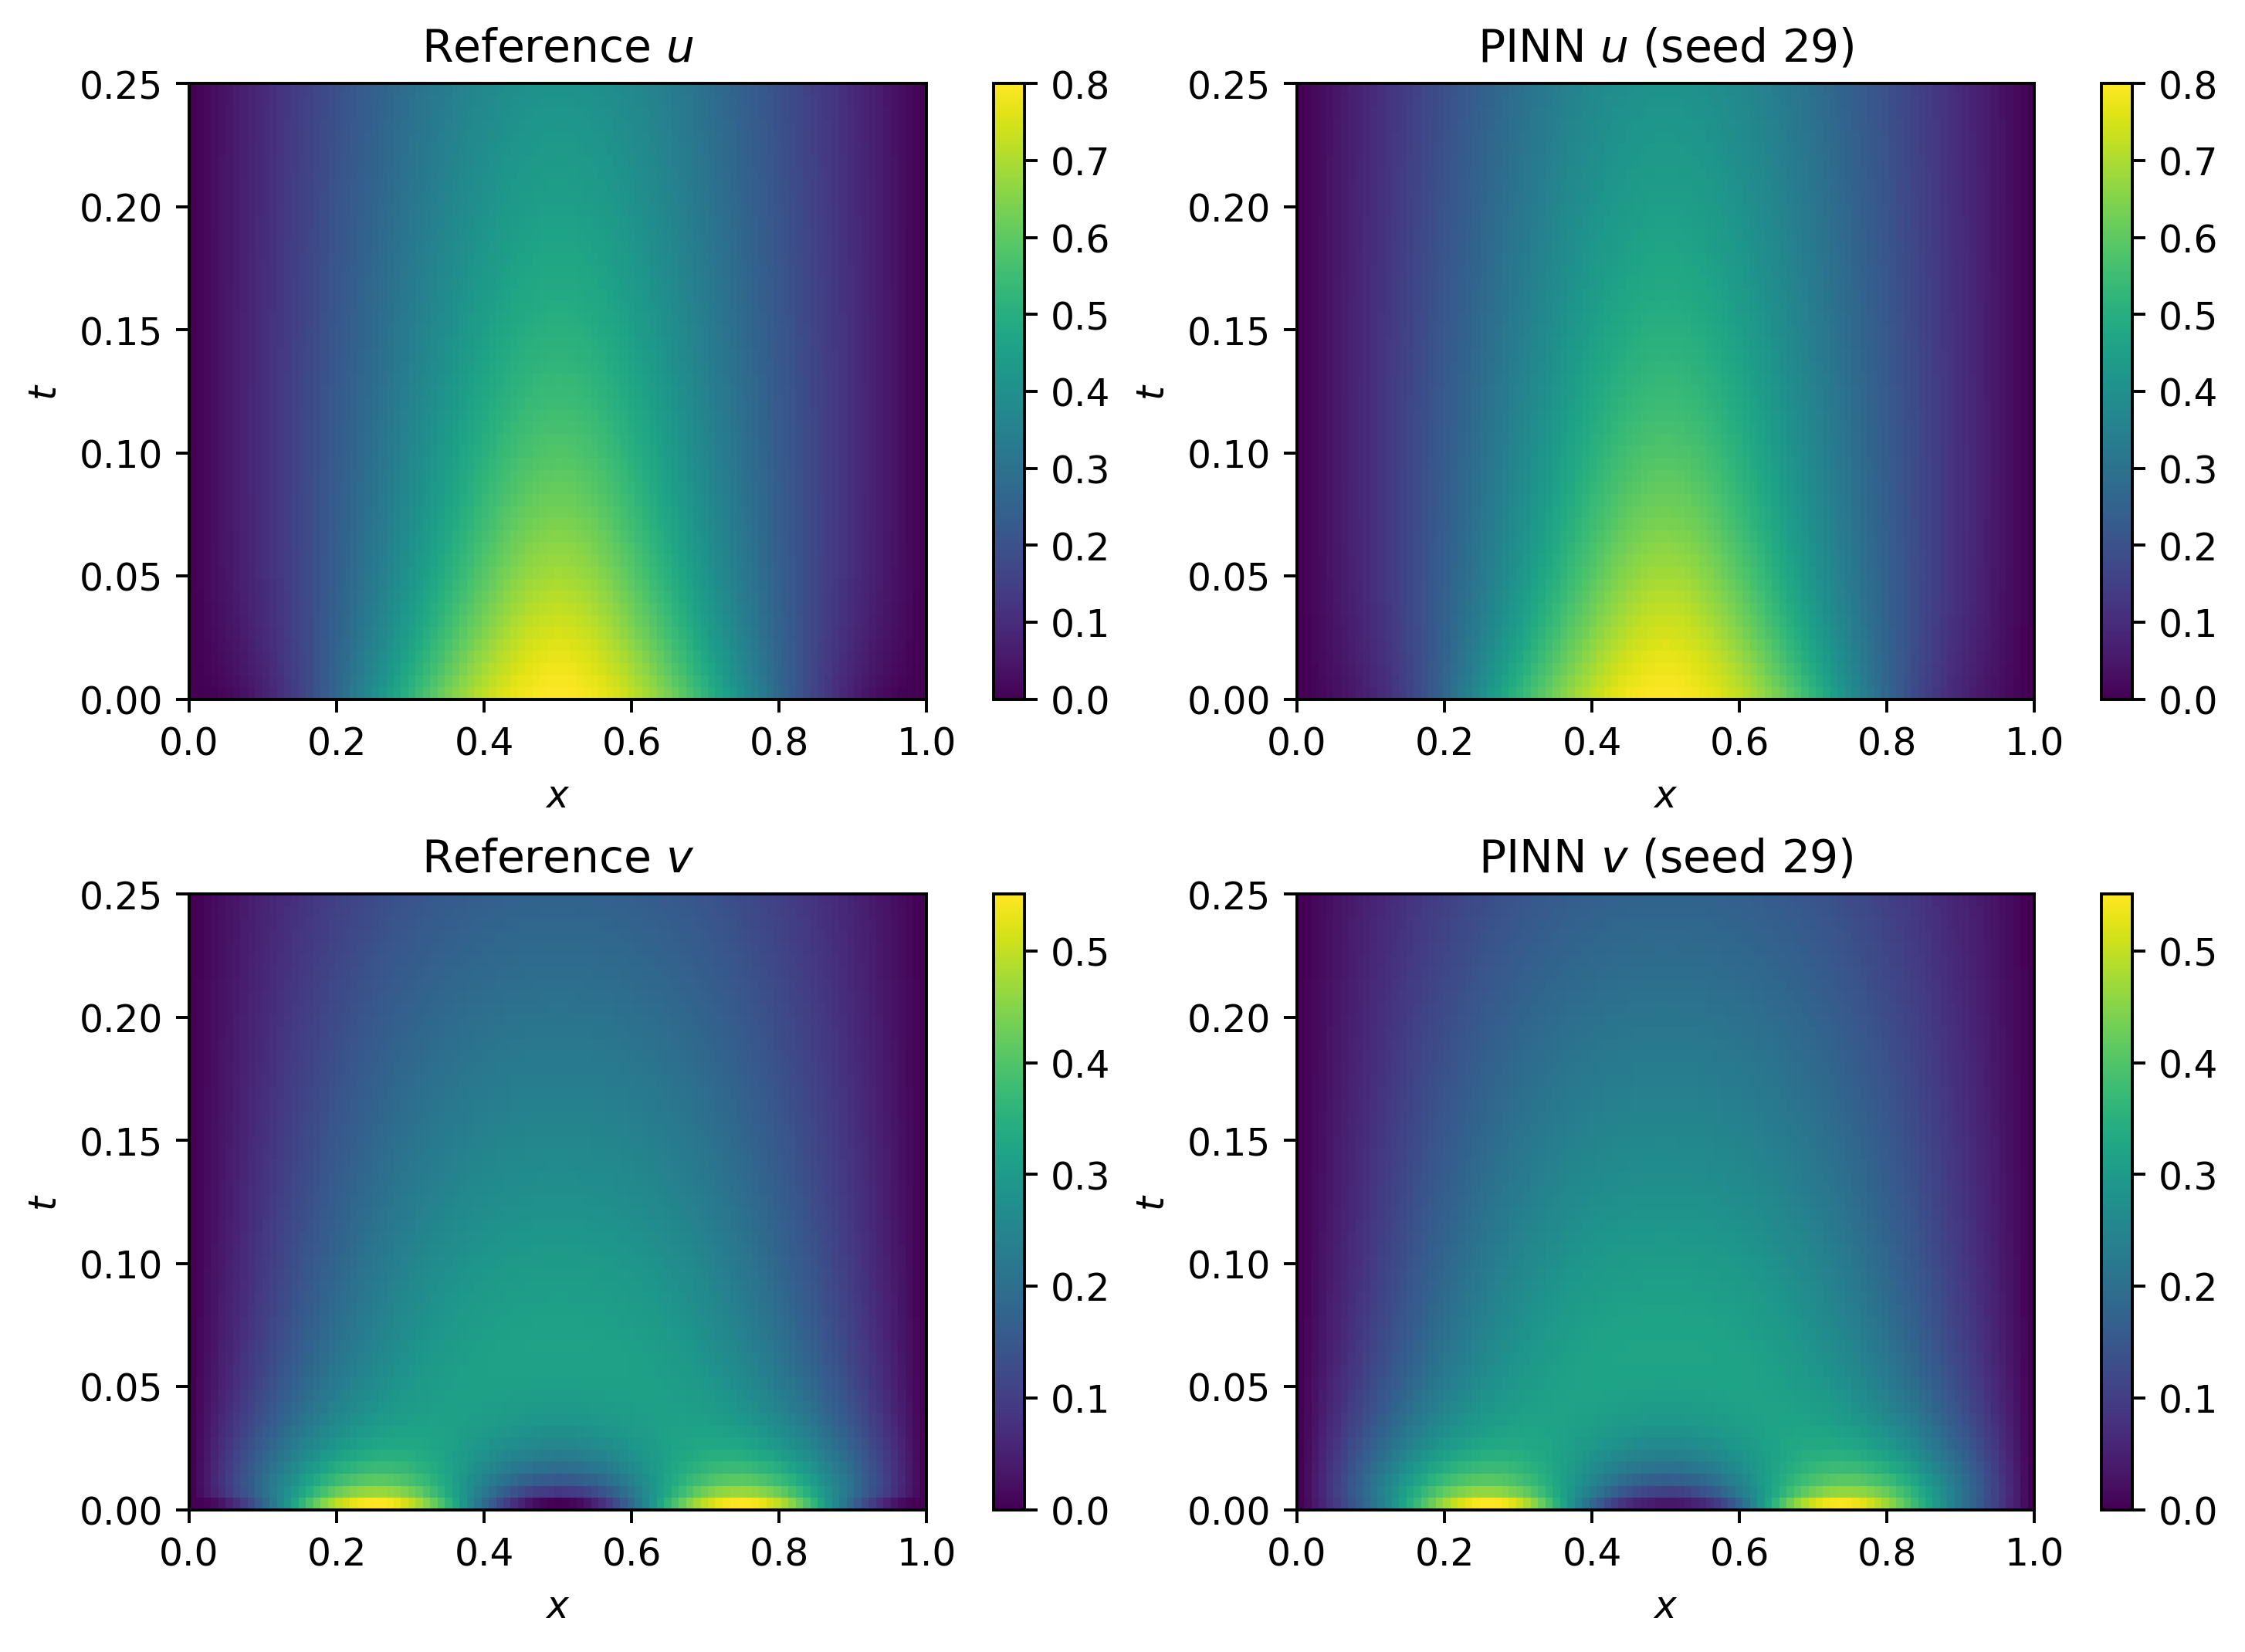
\includegraphics[width=0.90\textwidth]{figures/reproducible_solution_comparison.png}
\caption{Reference and median-RMSE PINN fields (seed 29). Within each component, the reference and PINN panels use exactly the same colour scale, so amplitude differences are not masked by independent normalization.}
\label{fig:computed-comparison}
\end{figure}

To avoid hiding componentwise discrepancies behind the global RMSE, Figures~\ref{fig:classical-error-comparison} and~\ref{fig:pinn-error-comparison} report absolute-error fields for \emph{both} components. FDM and FEM share a common scale within each component so that the two classical discretizations can be compared directly. The PINN errors are displayed separately because their magnitude is roughly two orders larger; forcing all methods onto one scale would visually erase the classical error structure. The corresponding componentwise RMSE values are
\[
\begin{array}{c|cc}
\text{Method} & \operatorname{RMSE}(u) & \operatorname{RMSE}(v)\\ \hline
\text{FDM} & 6.966\times10^{-5} & 1.733\times10^{-4}\\
\text{FEM} & 4.723\times10^{-5} & 1.162\times10^{-4}\\
\text{PINN (seed 29)} & 1.848\times10^{-3} & 4.154\times10^{-3}.
\end{array}
\]
Thus the larger classical-solver error occurs in the second component, a feature that was not visible when only first-component error maps were displayed. FEM remains the most accurate classical method in both components for this benchmark, while the PINN discrepancy is one to two orders of magnitude larger on the common grid.

\begin{figure}[!htbp]
\centering
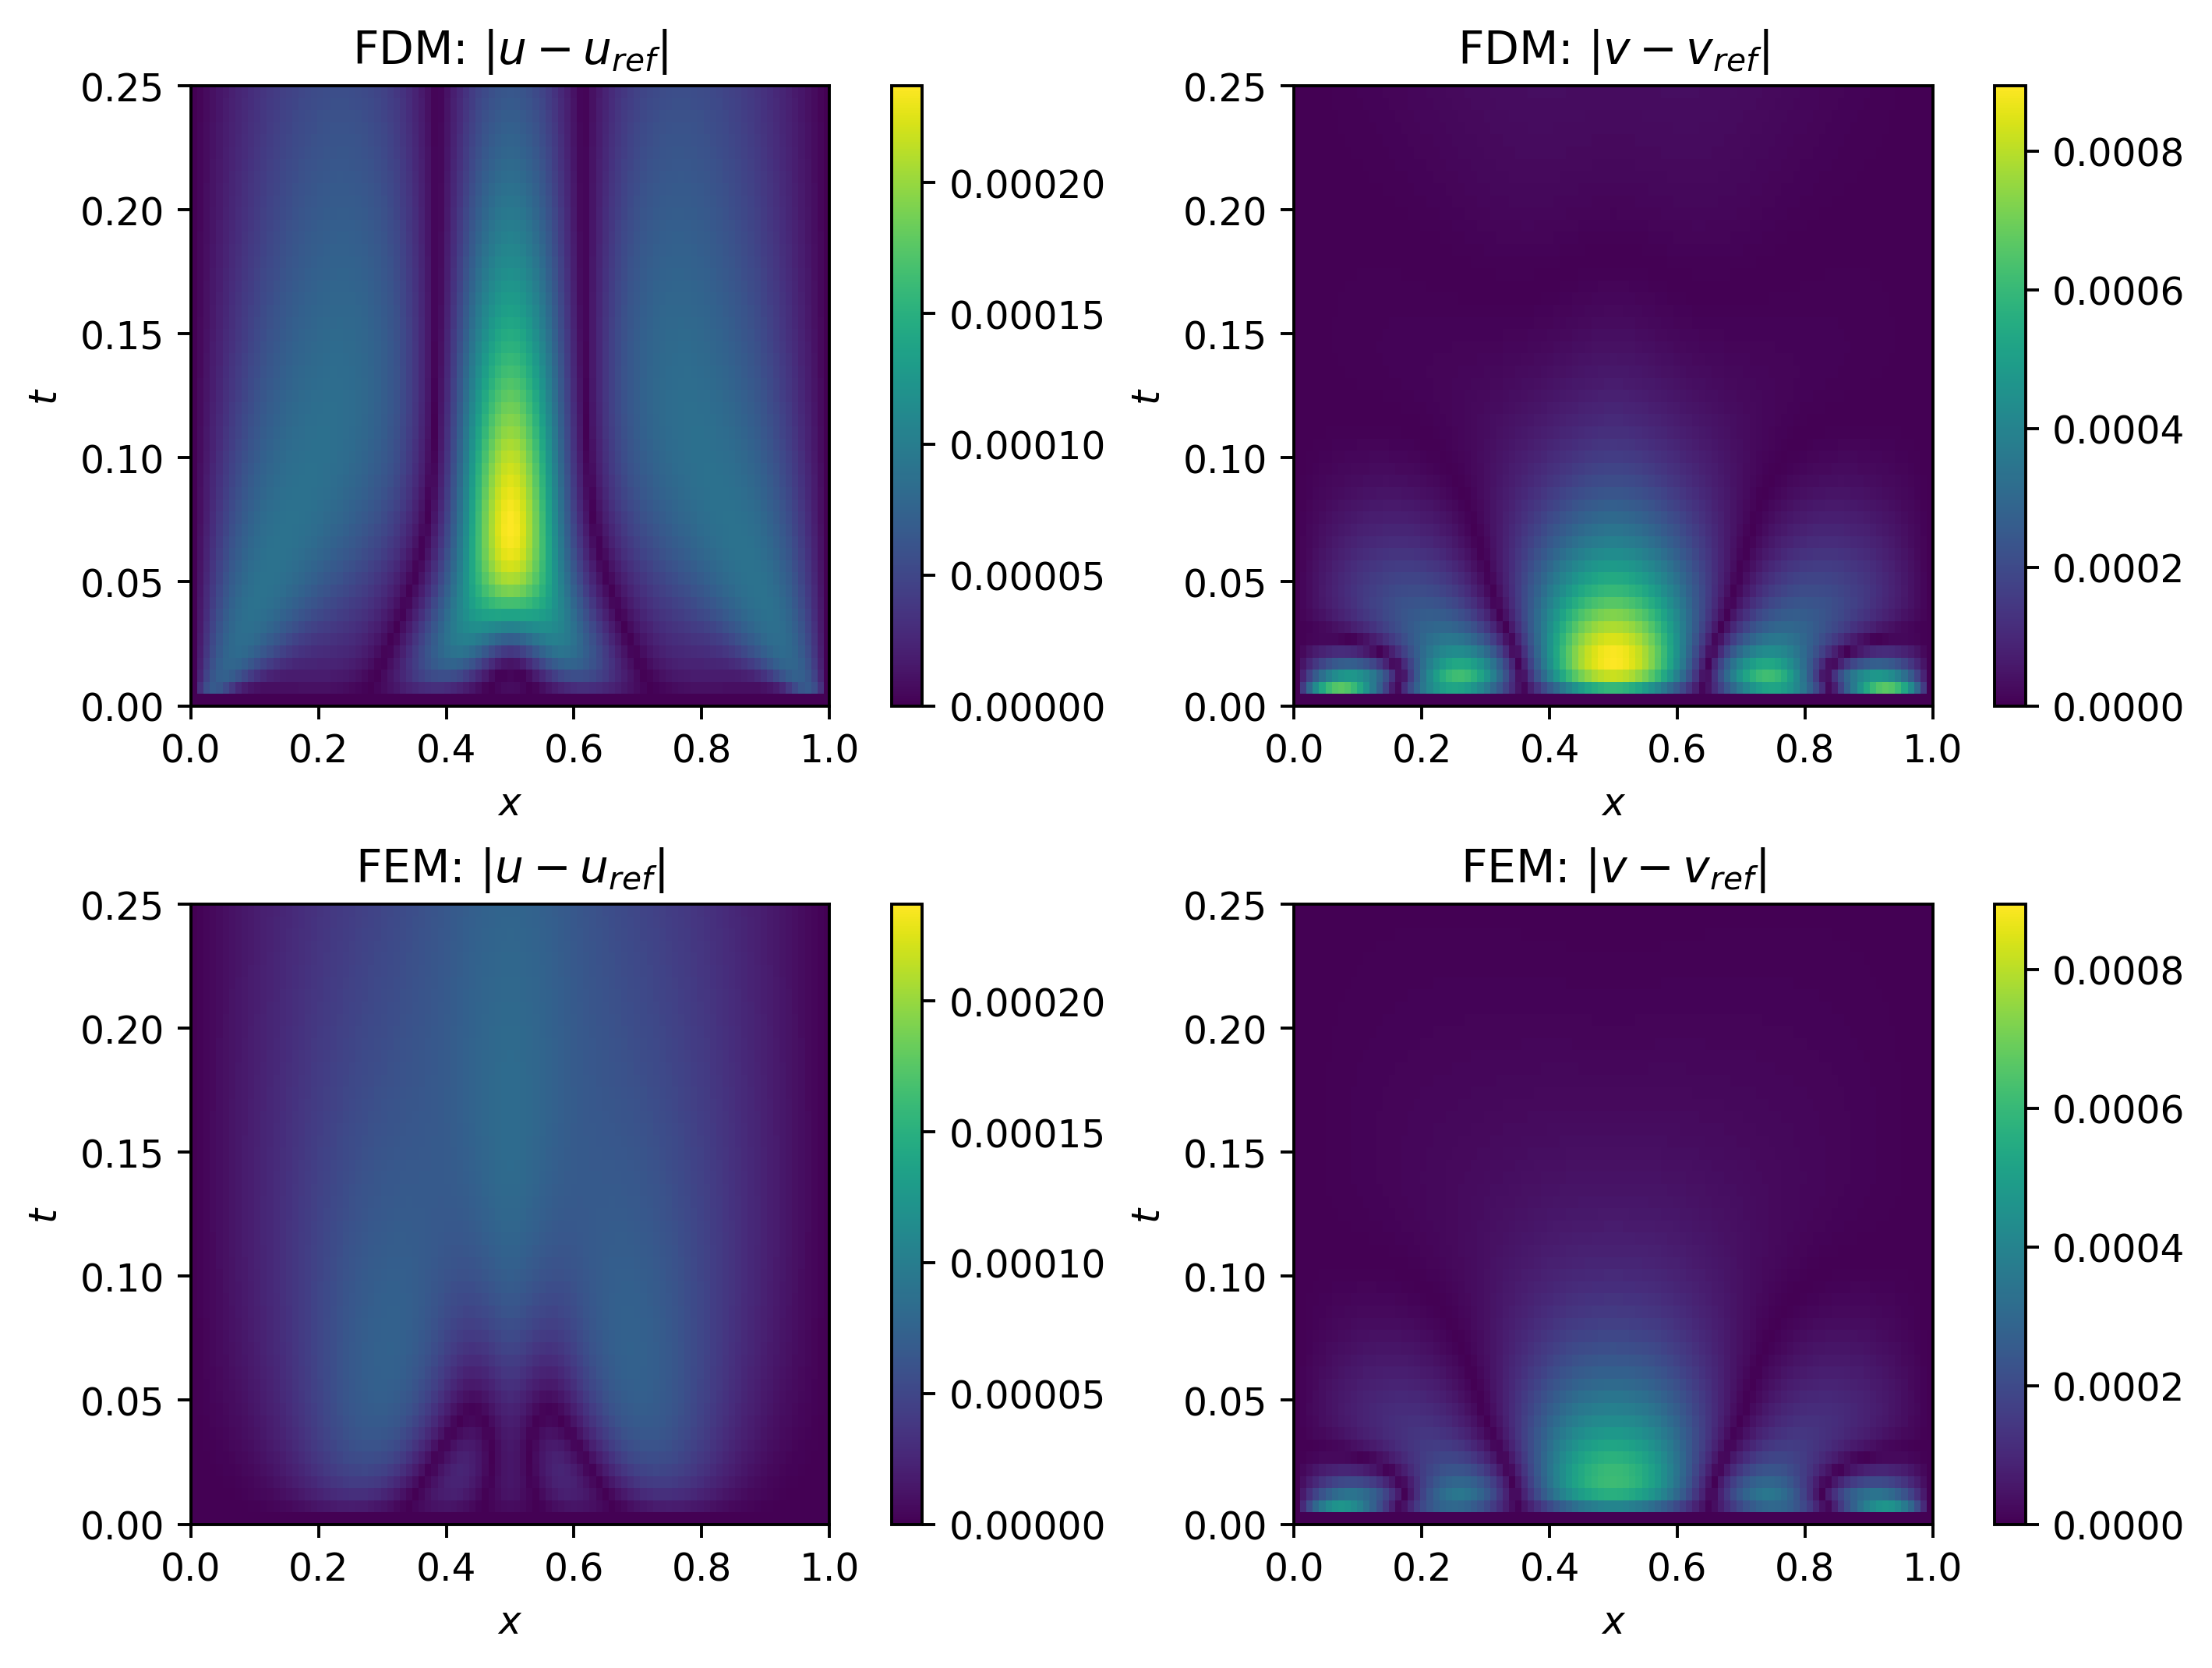
\includegraphics[width=0.88\textwidth]{figures/reproducible_classical_error_comparison.png}
\caption{Absolute error fields for the classical discretizations relative to the refined reference. Both components are shown. For each component, FDM and FEM use the same colour scale, so their error magnitudes can be compared directly without method-specific normalization.}
\label{fig:classical-error-comparison}
\end{figure}

\begin{figure}[!htbp]
\centering
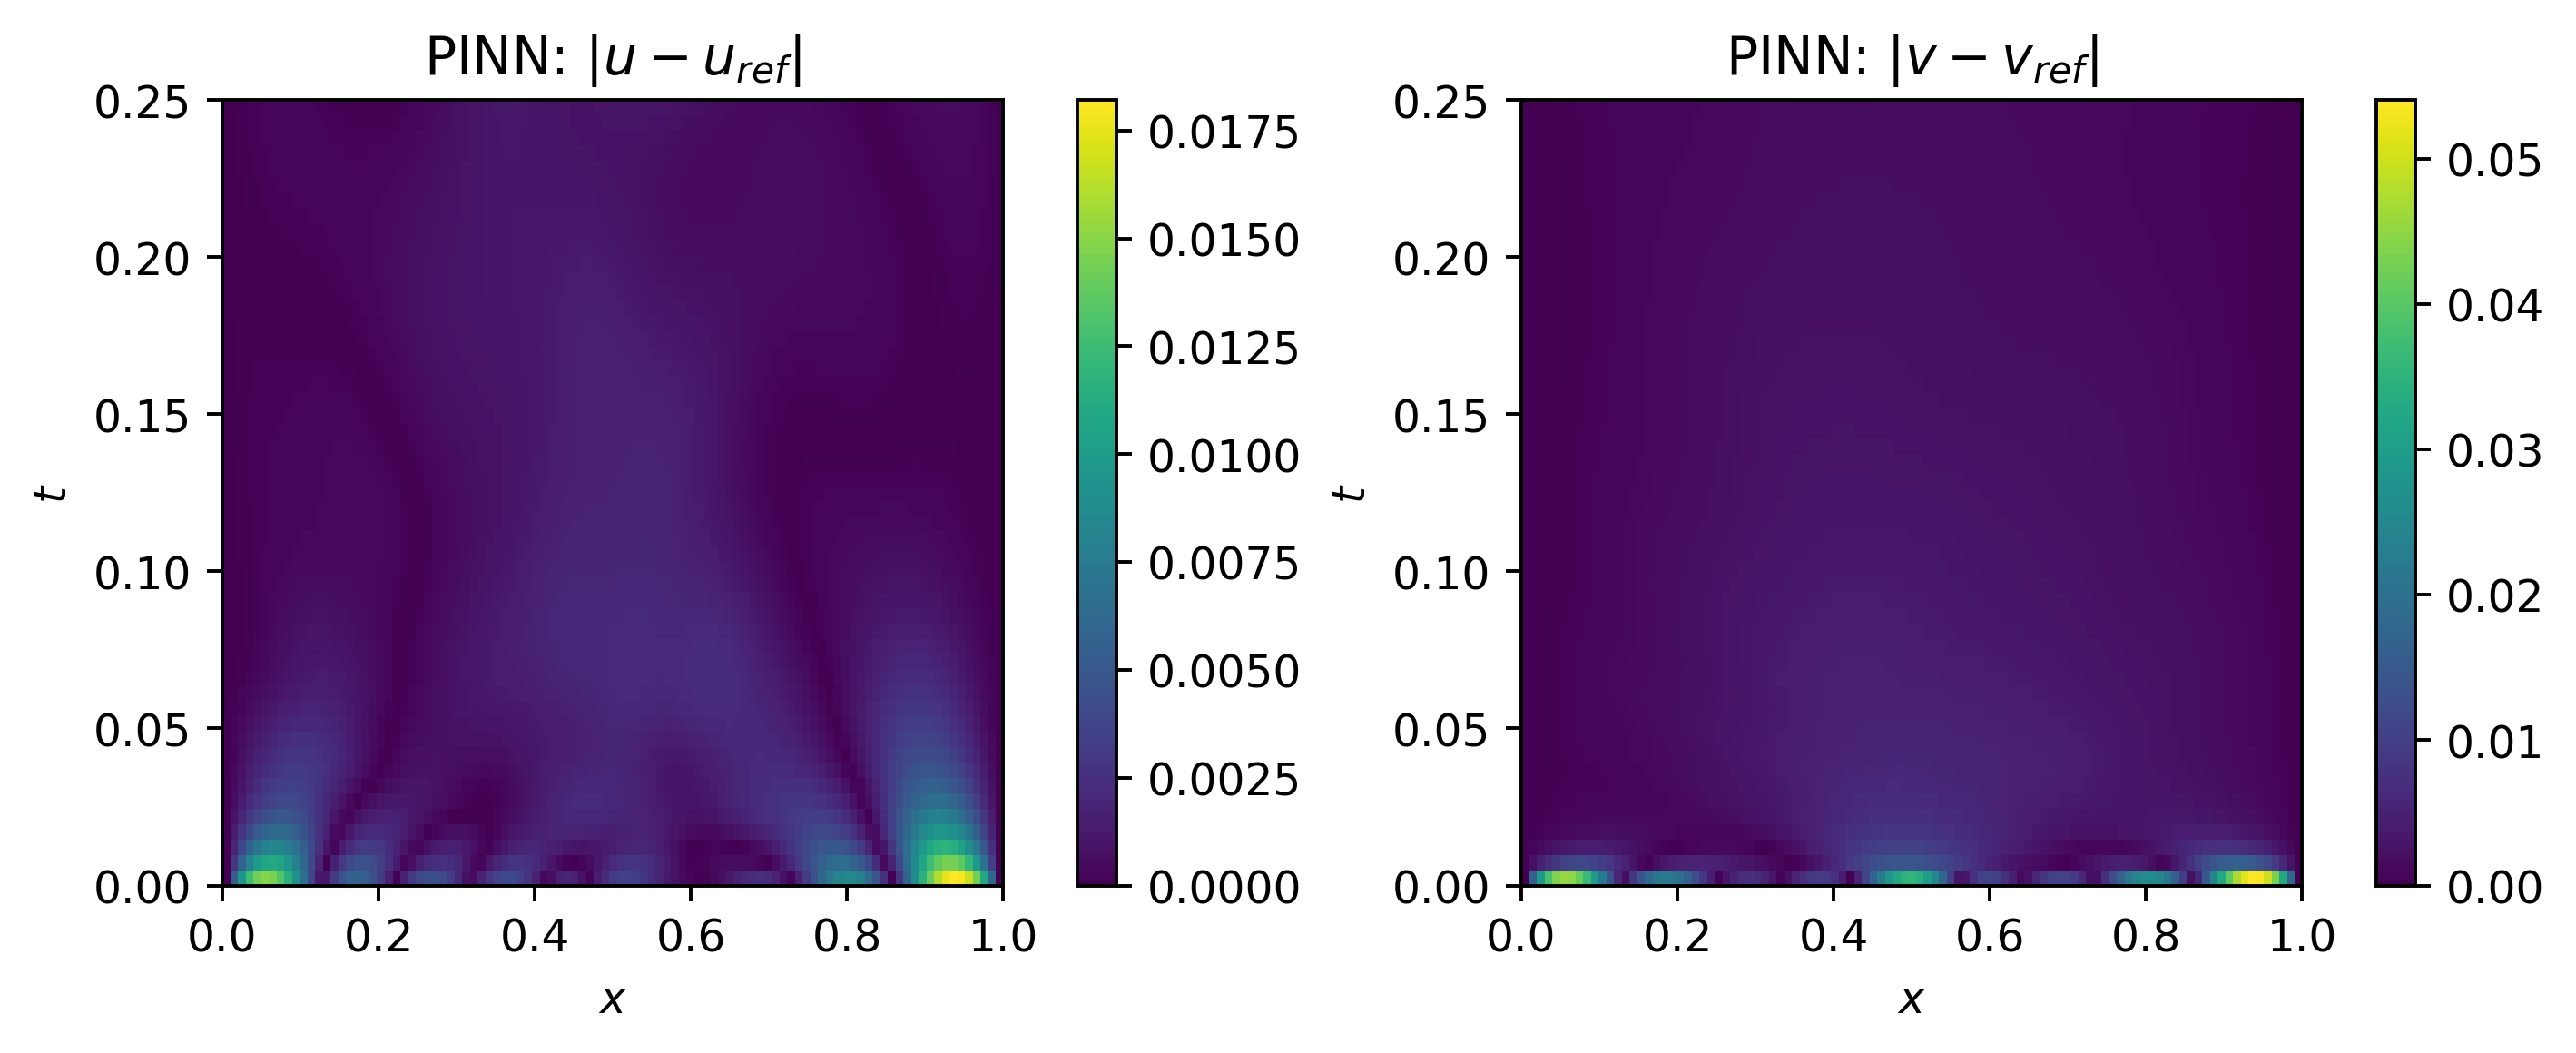
\includegraphics[width=0.88\textwidth]{figures/reproducible_pinn_error_comparison.png}
\caption{Absolute error fields for the median-RMSE PINN realization (seed 29). The colour bars are displayed explicitly for each component because the PINN errors are roughly two orders of magnitude larger than the classical-solver errors; using a single scale for all methods would make the FDM/FEM error structure visually indistinguishable.}
\label{fig:pinn-error-comparison}
\end{figure}

The classical error maps in Figure~\ref{fig:classical-error-comparison} show that the second component is more difficult for both discretizations, consistently with the componentwise RMSE values above. FEM has the smaller error in both $u$ and $v$. Figure~\ref{fig:pinn-error-comparison} makes the larger PINN discrepancies visible without rescaling the classical maps to the neural-error range. The PINN error is most pronounced during the early high-gradient part of the evolution and is larger for $v$ than for $u$. This is compatible with the difficulty of optimizing residuals containing first- and second-order derivatives, but the present experiment does not isolate curvature or any single loss component as the cause. It is an interpretation of this benchmark, not evidence that the same ordering must hold for nonsmooth, inverse, or higher-dimensional problems.

Figure~\ref{fig:temporal-snapshots} compares both components at three times. It complements the global and componentwise RMSE by checking that agreement is not confined to the terminal state or obscured by a space--time average. Because the absolute errors are small relative to the field amplitudes, the profiles can appear visually close even when the PINN RMSE is substantially larger; Figures~\ref{fig:classical-error-comparison}--\ref{fig:pinn-error-comparison} make that difference explicit.

\begin{figure}[!htbp]
\centering
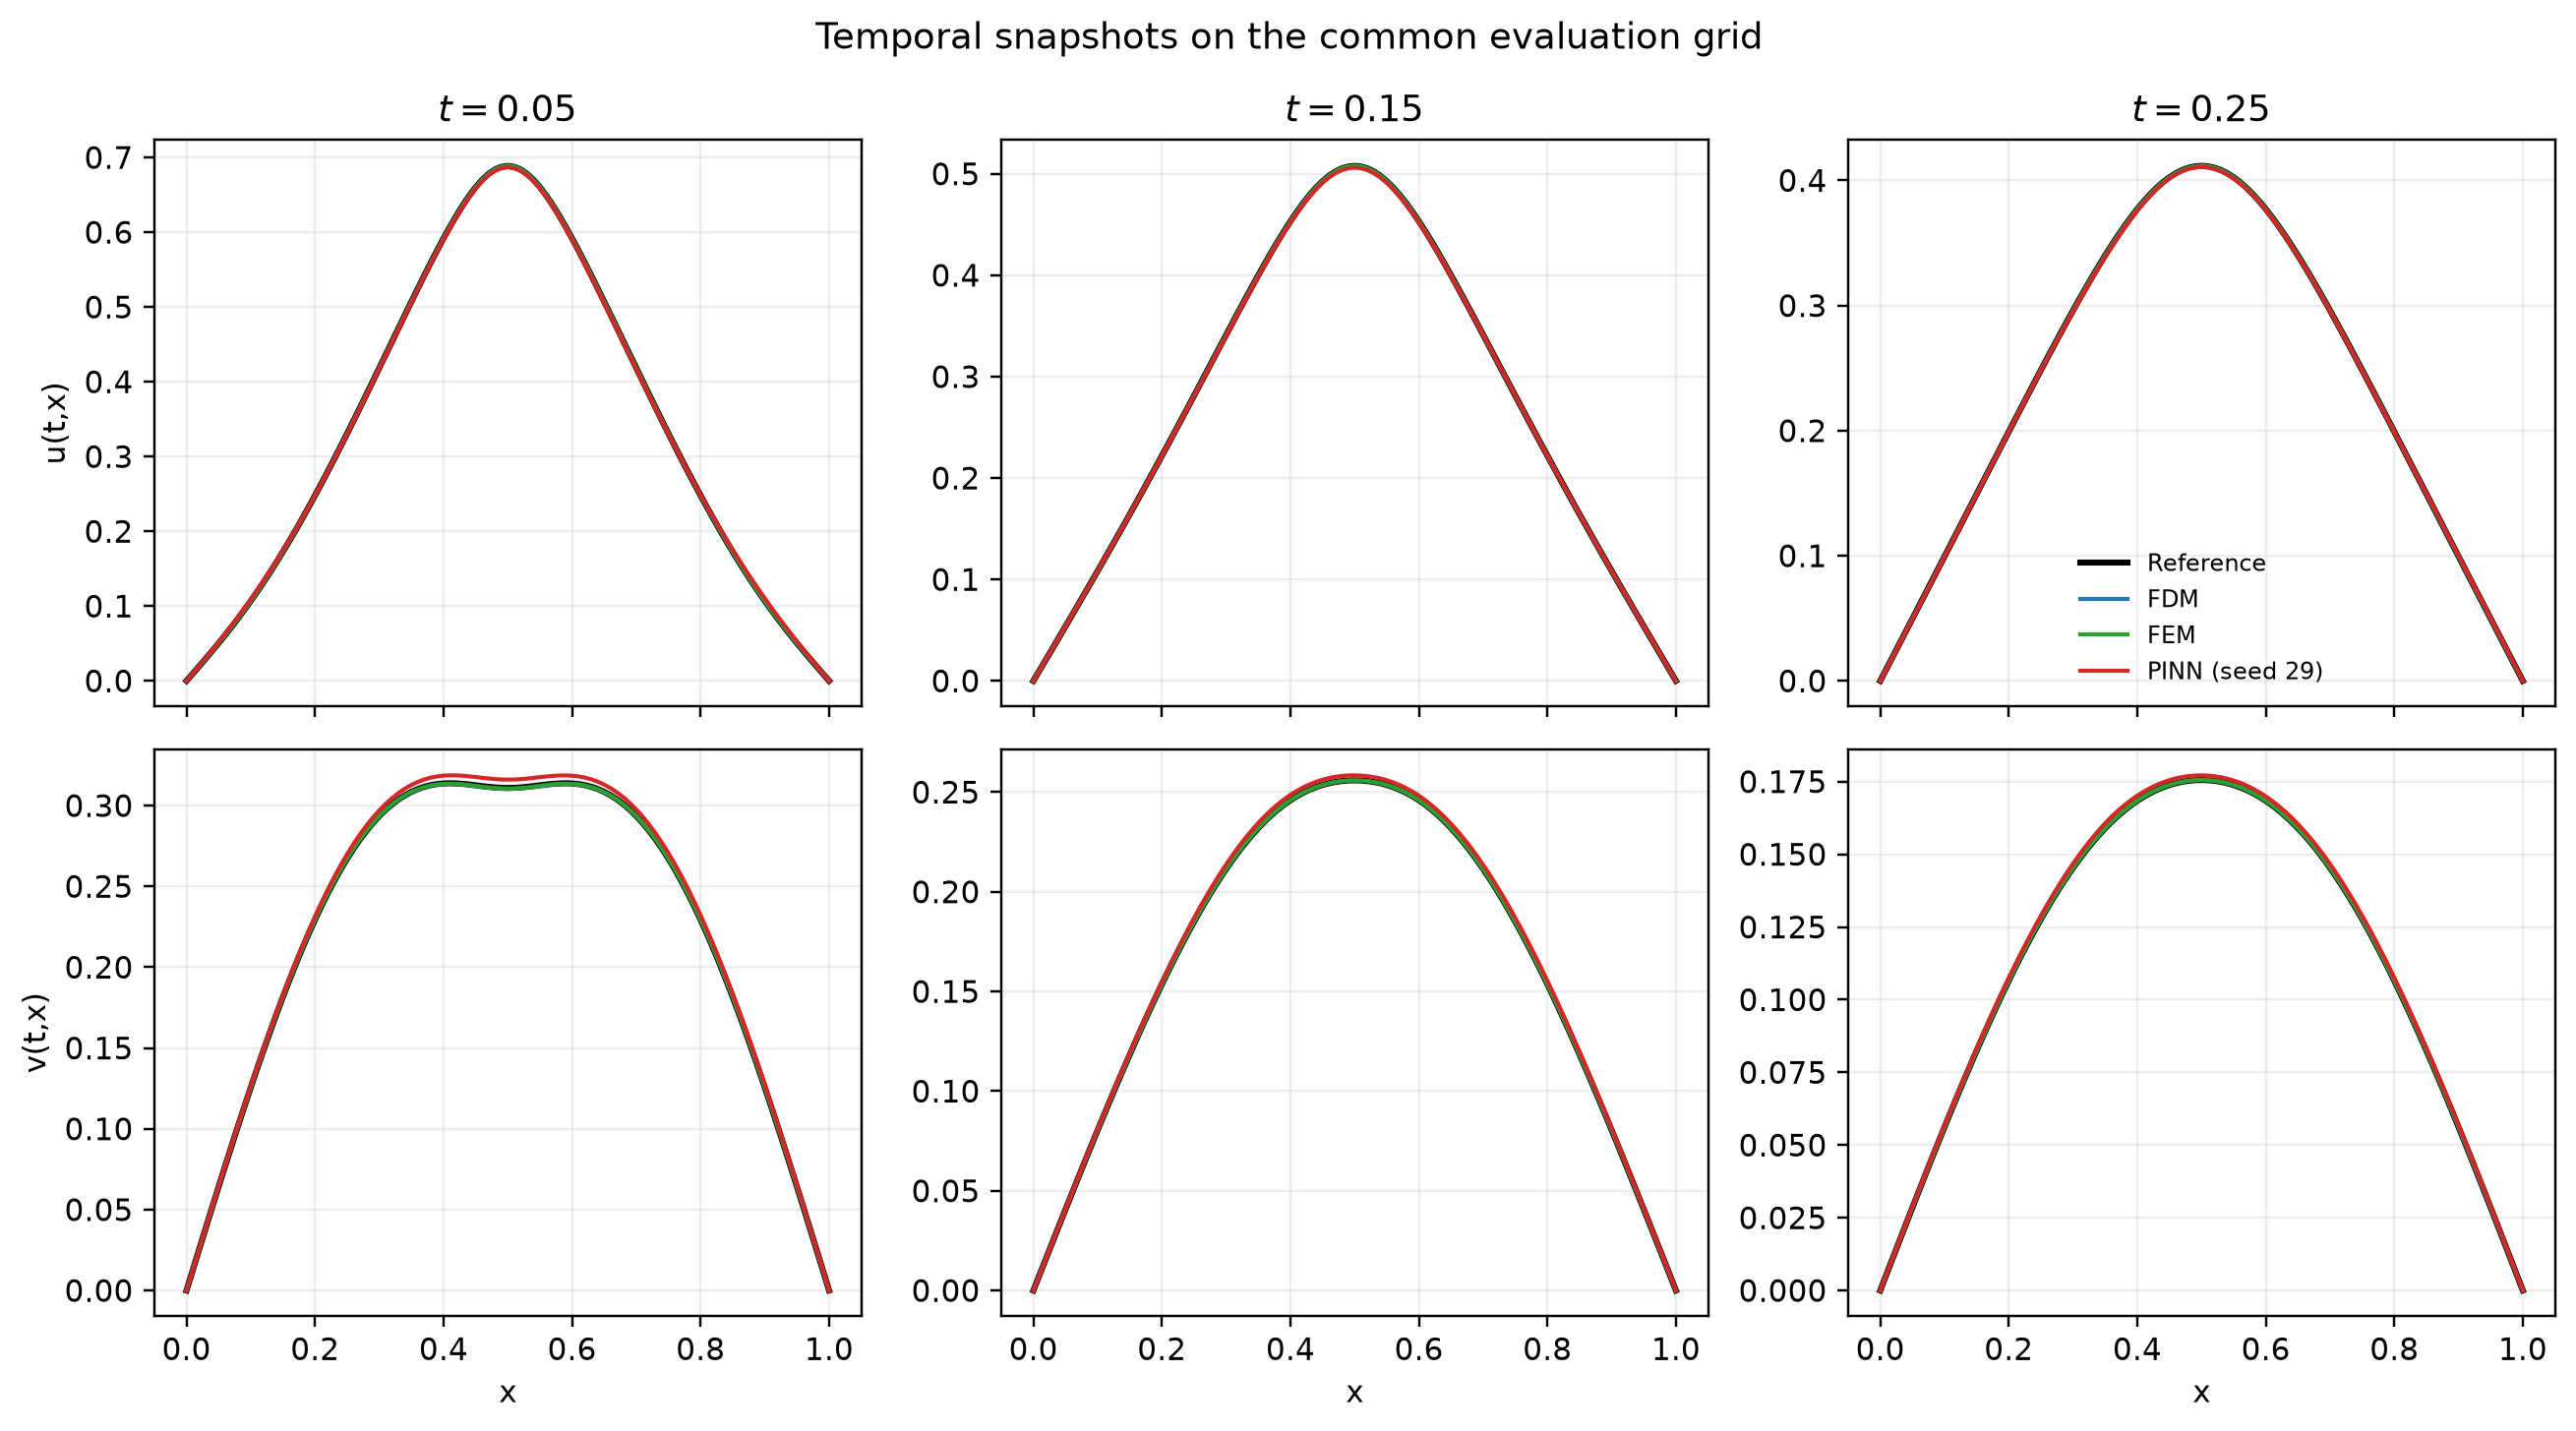
\includegraphics[width=\textwidth]{figures/reproducible_temporal_snapshots.png}
\caption{Temporal snapshots of both components for the reference, FDM, FEM, and the median-RMSE PINN realization (seed 29).}
\label{fig:temporal-snapshots}
\end{figure}

The reference profiles show the combined action of diffusion, boundary loss, and nonlinear dissipation. The maximum of $u$ decreases from $0.8$ initially to $0.689$, $0.508$, and $0.412$ at $t=0.05$, $0.15$, and $0.25$, respectively, while remaining centred near $x=0.5$. The initially two-peaked profile of $v$ is rapidly smoothed and becomes a single broad central profile; its maximum is approximately $0.314$, $0.256$, and $0.176$ at the same times. Thus the transfer term does not generate sustained growth of $v$ on this parameter range: diffusion, boundary flux, and the sink $-v|v_x|^2$ dominate its integrated evolution. Agreement improves as the profiles become smoother: the instantaneous combined RMSE decreases from $1.85\times10^{-4}$ at $t=0.05$ to $3.31\times10^{-5}$ at $t=0.25$ for FDM, from $1.19\times10^{-4}$ to $3.35\times10^{-5}$ for FEM, and from $2.68\times10^{-3}$ to $9.58\times10^{-4}$ for the median-RMSE PINN (seed 29). This temporal decrease partly reflects the parabolic damping of high-gradient features and should not be interpreted as a convergence rate.


\subsection{Manufactured-solution verification of FDM and FEM}
\label{subsec:mms-results}

Table~\ref{tab:mms-spatial} reports independent spatial refinements for the forced problem of Section~\ref{subsec:mms}. The RMSE order is computed as $p=\log_2(E_h/E_{h/2})$. Both implementations recover the expected quadratic spatial behaviour on this smooth test: FDM orders range from $1.984$ to $1.993$, while the $P_1$ FEM orders range from $1.996$ to $2.001$.

\begin{table}[!htbp]
\centering
\caption{Manufactured-solution spatial verification at $T=0.02$.}
\label{tab:mms-spatial}
\begin{tabular}{lrrr}
\toprule
Method & Resolution & RMSE & Observed order\\
\midrule
FDM & 51  & $6.6232\times10^{-4}$ & --\\
FDM & 101 & $1.6653\times10^{-4}$ & 1.992\\
FDM & 201 & $4.1840\times10^{-5}$ & 1.993\\
FDM & 401 & $1.0575\times10^{-5}$ & 1.984\\
\midrule
FEM & 50 elements  & $1.1038\times10^{-4}$ & --\\
FEM & 100 elements & $2.7665\times10^{-5}$ & 1.996\\
FEM & 200 elements & $6.9221\times10^{-6}$ & 1.999\\
FEM & 400 elements & $1.7298\times10^{-6}$ & 2.001\\
\bottomrule
\end{tabular}
\end{table}

Temporal refinement gives first-order behaviour when the spatial discretization is made sufficiently fine. For FDM, the observed orders over $\Delta t=8,4,2,1\times10^{-4}$ are $0.983$, $0.973$, and $0.951$; for FEM they are $0.996$, $0.999$, and $1.000$. Figure~\ref{fig:mms-verification} displays both independent refinement studies. The purpose is implementation verification: unlike the coupled reference-refinement plot used elsewhere in the paper, $h$ and $\Delta t$ are varied separately.

\begin{figure}[!htbp]
\centering
\begin{subfigure}{.48\textwidth}
\centering
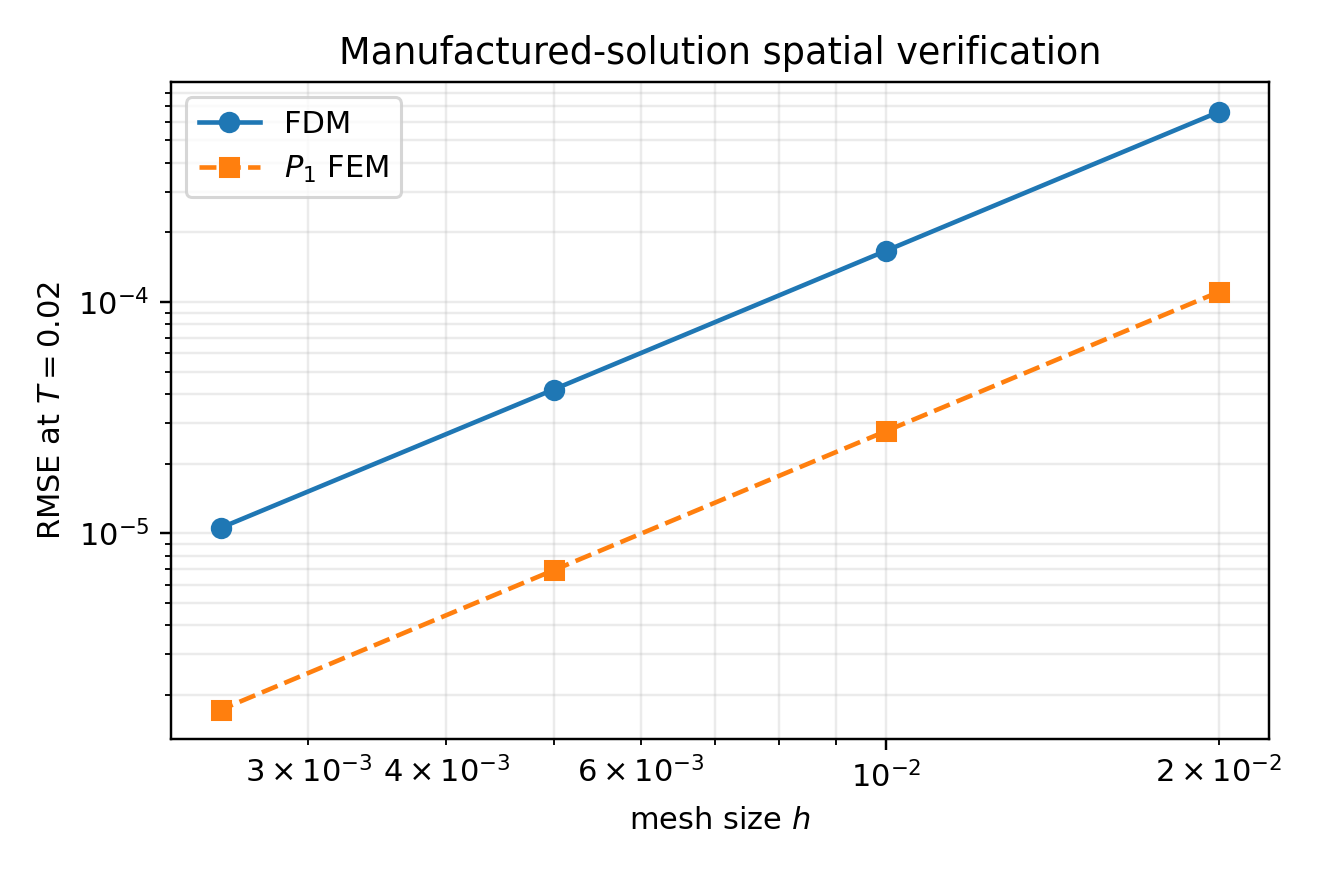
\includegraphics[width=\textwidth]{figures/mms_spatial_convergence.png}
\caption{Spatial refinement.}
\end{subfigure}\hfill
\begin{subfigure}{.48\textwidth}
\centering
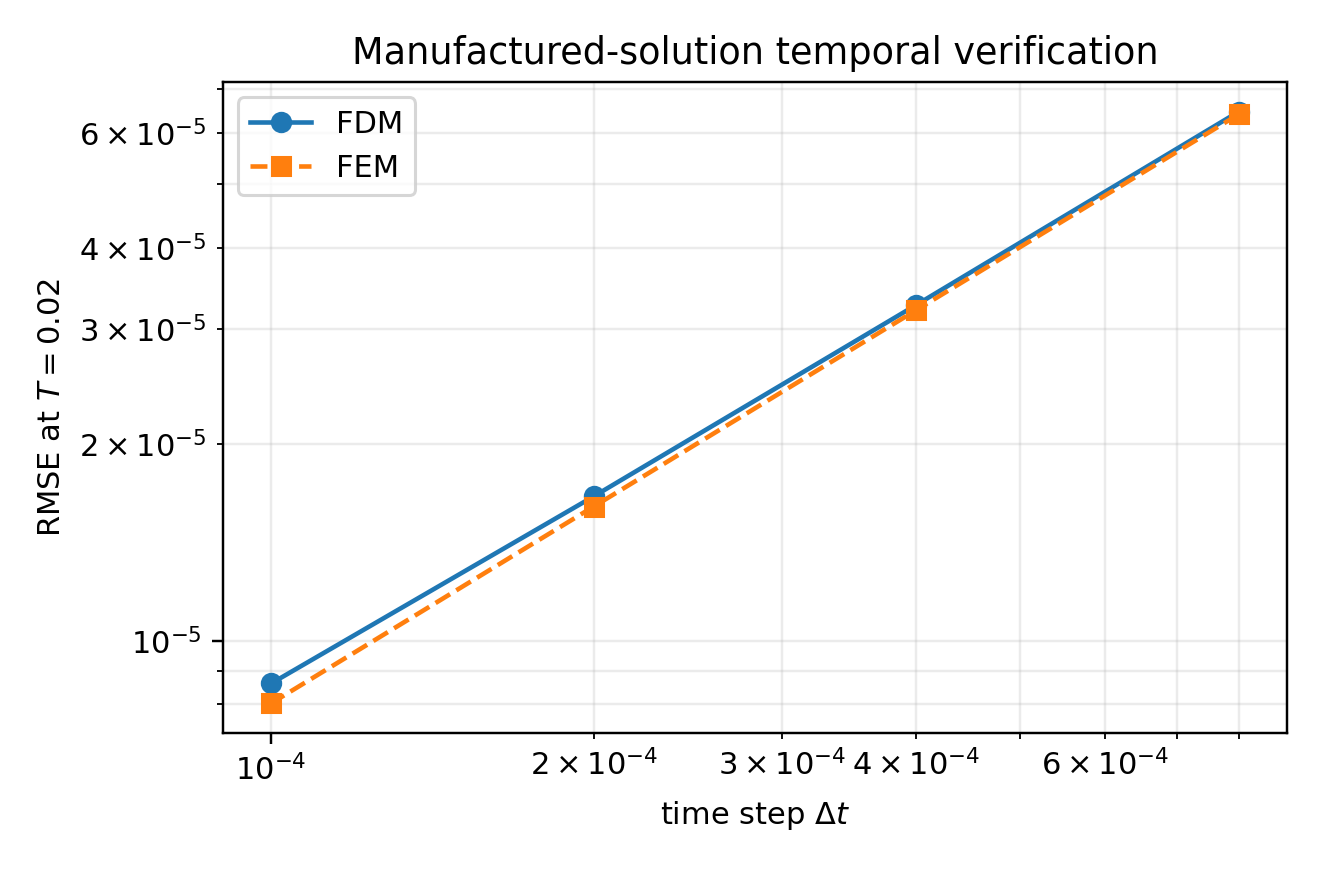
\includegraphics[width=\textwidth]{figures/mms_temporal_convergence.png}
\caption{Temporal refinement.}
\end{subfigure}
\caption{Manufactured-solution verification of the classical discretizations.}
\label{fig:mms-verification}
\end{figure}

\subsection{Three-component non-monotone benchmark}
\label{subsec:three-results}

The three-component problem complements the analytical non-monotone example with a controlled numerical realization in which the two preceding-gradient estimates are available independently. Against the $401$-point reference, FDM attains RMSE $1.484\times10^{-4}$ and relative $L^2$ error $6.110\times10^{-4}$, whereas FEM attains RMSE $1.136\times10^{-4}$ and relative $L^2$ error $4.677\times10^{-4}$. Componentwise errors are reported in Table~\ref{tab:three-component}. No positive increment is observed for any of the three trapezoidal partial masses on the common grid, and both discretizations remain nonnegative up to floating-point roundoff.

\begin{table}[!htbp]
\centering
\caption{Three-component benchmark: errors against the refined reference.}
\label{tab:three-component}
{\small
\setlength{\tabcolsep}{3pt}
\begin{tabular}{@{}lccccc@{}}
\toprule
Method & RMSE & Rel. $L^2$ & $u$ RMSE & $v$ RMSE & $w$ RMSE\\
\midrule
FDM & $1.484\mathrm{e}{-4}$ & $6.110\mathrm{e}{-4}$ & $6.966\mathrm{e}{-5}$ & $1.885\mathrm{e}{-4}$ & $1.603\mathrm{e}{-4}$\\
FEM & $1.136\mathrm{e}{-4}$ & $4.677\mathrm{e}{-4}$ & $4.723\mathrm{e}{-5}$ & $1.509\mathrm{e}{-4}$ & $1.171\mathrm{e}{-4}$\\
\bottomrule
\end{tabular}
}
\end{table}

\begin{figure}[!htbp]
\centering
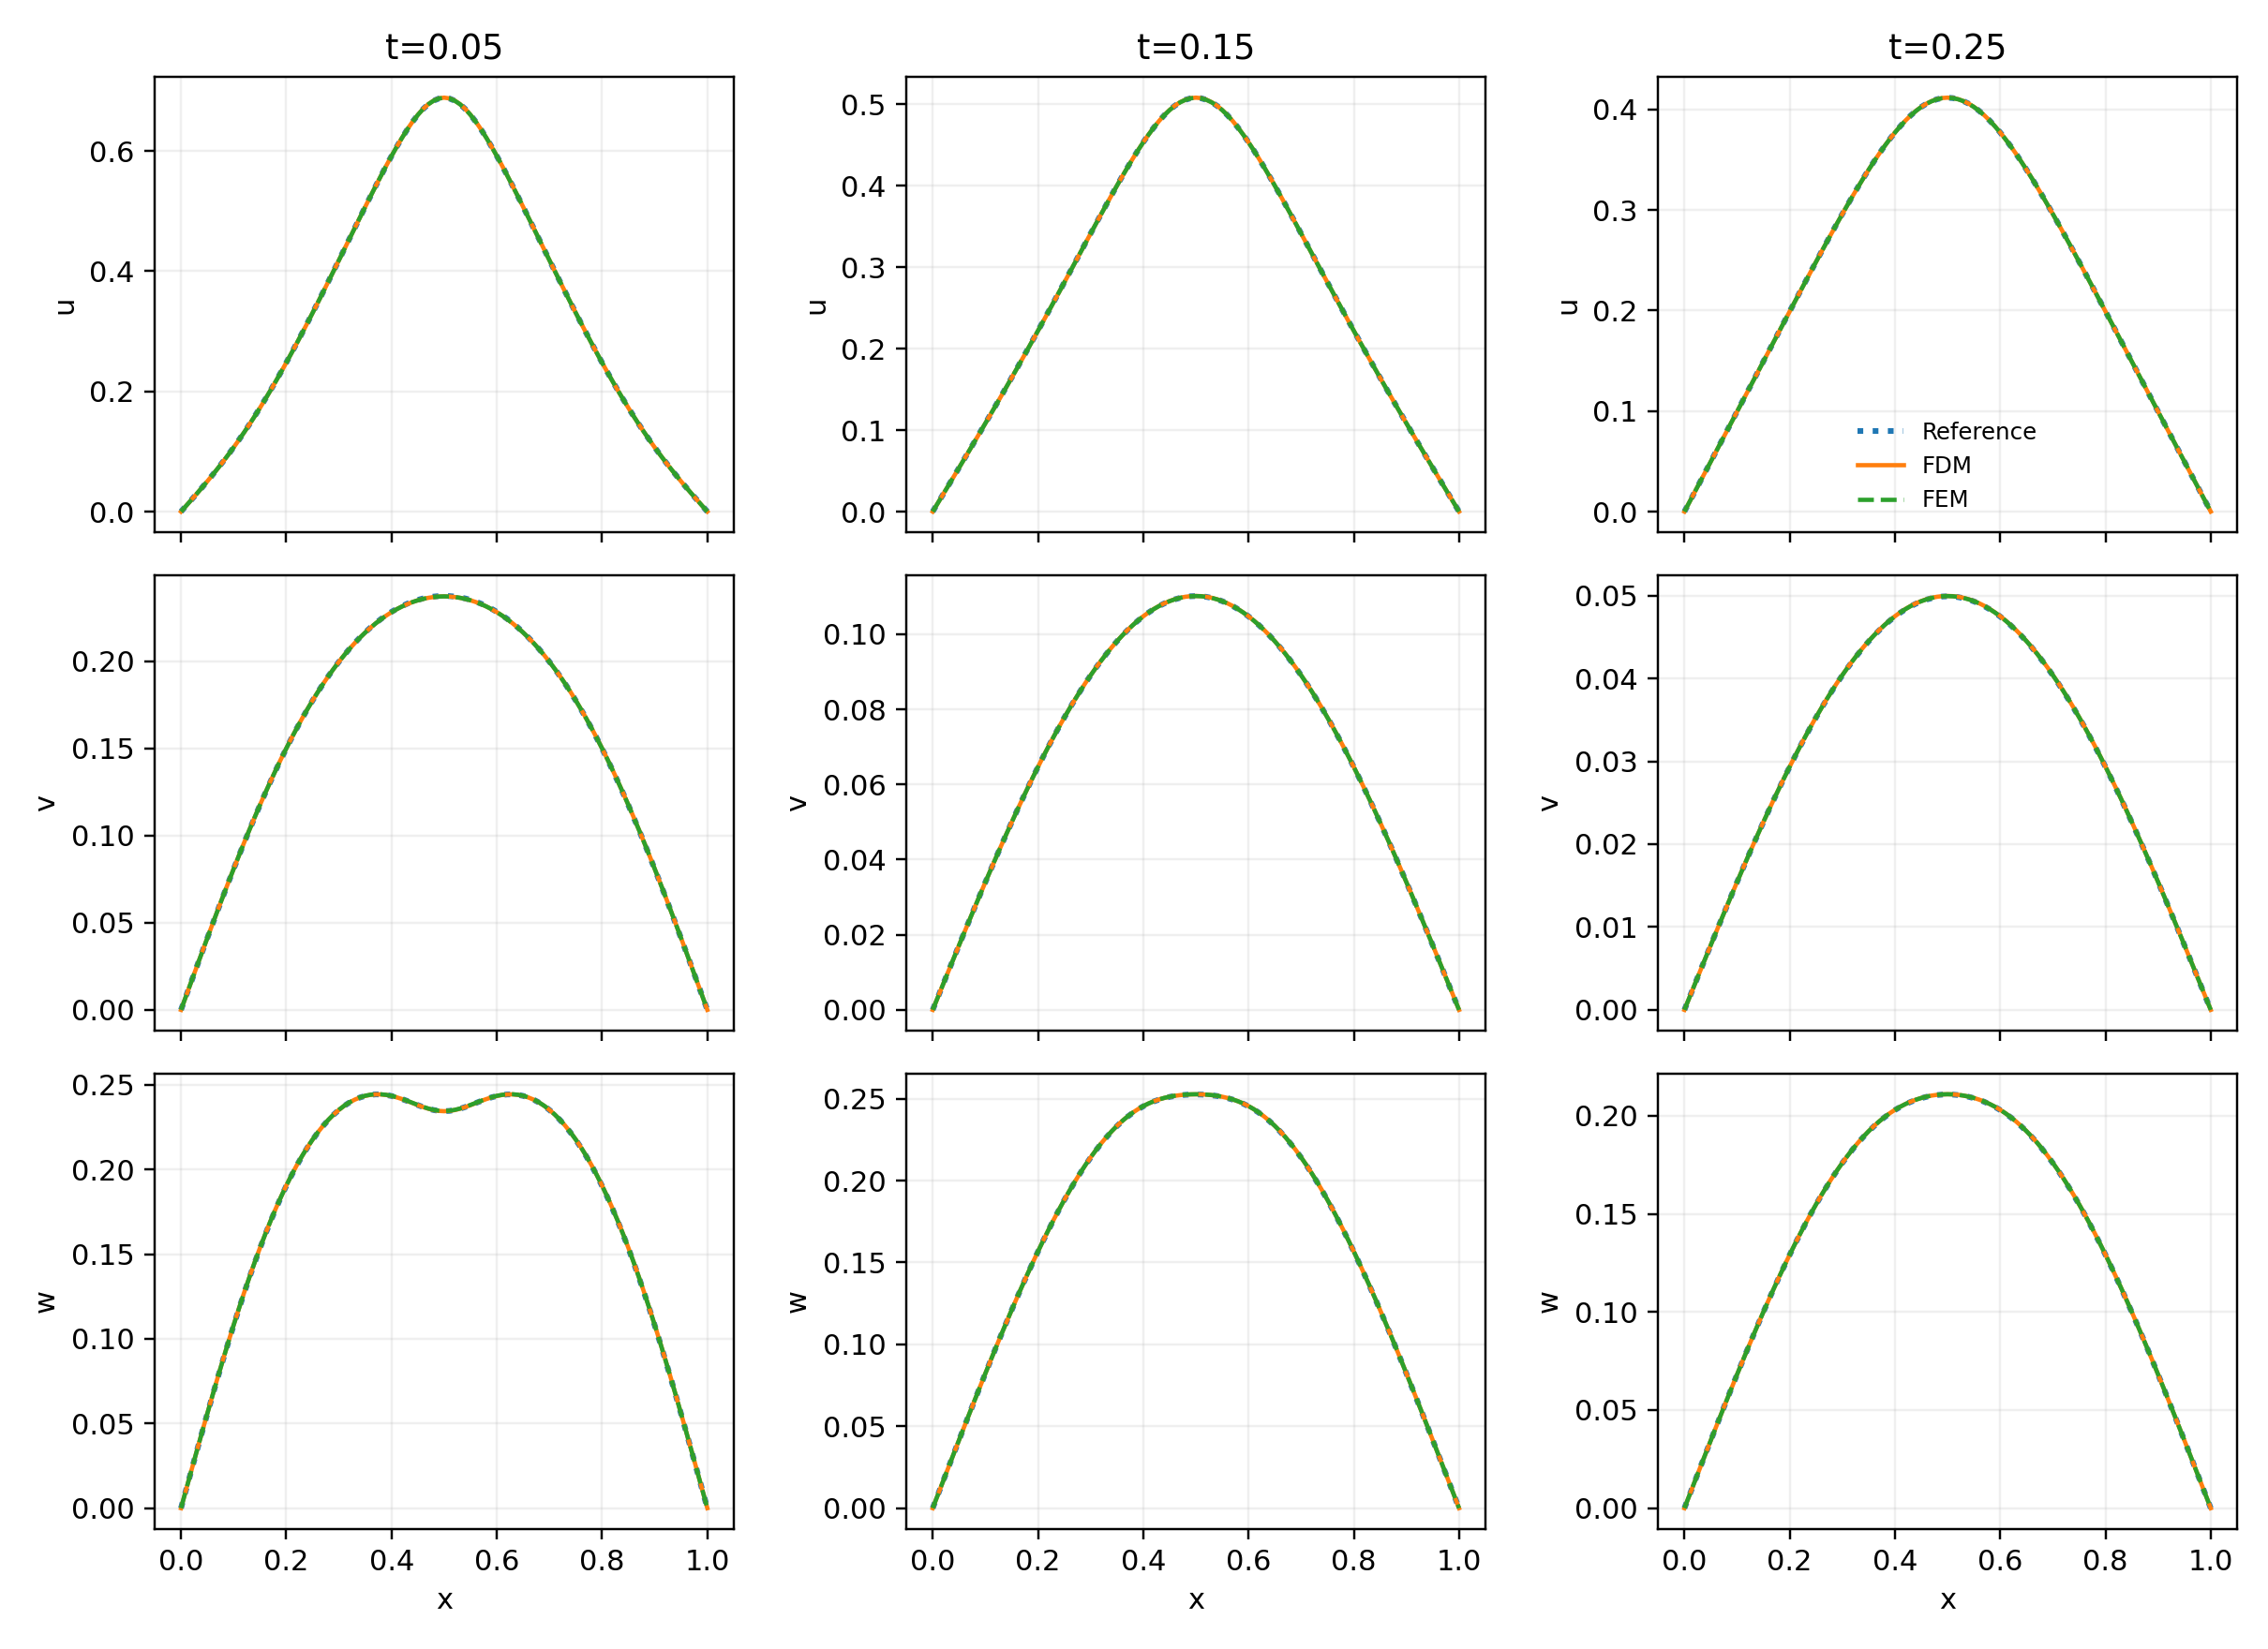
\includegraphics[width=.96\textwidth]{figures/three_component_snapshots.png}
\caption{Temporal snapshots for the three-component non-monotone benchmark.}
\label{fig:three-snapshots}
\end{figure}

\begin{figure}[!htbp]
\centering
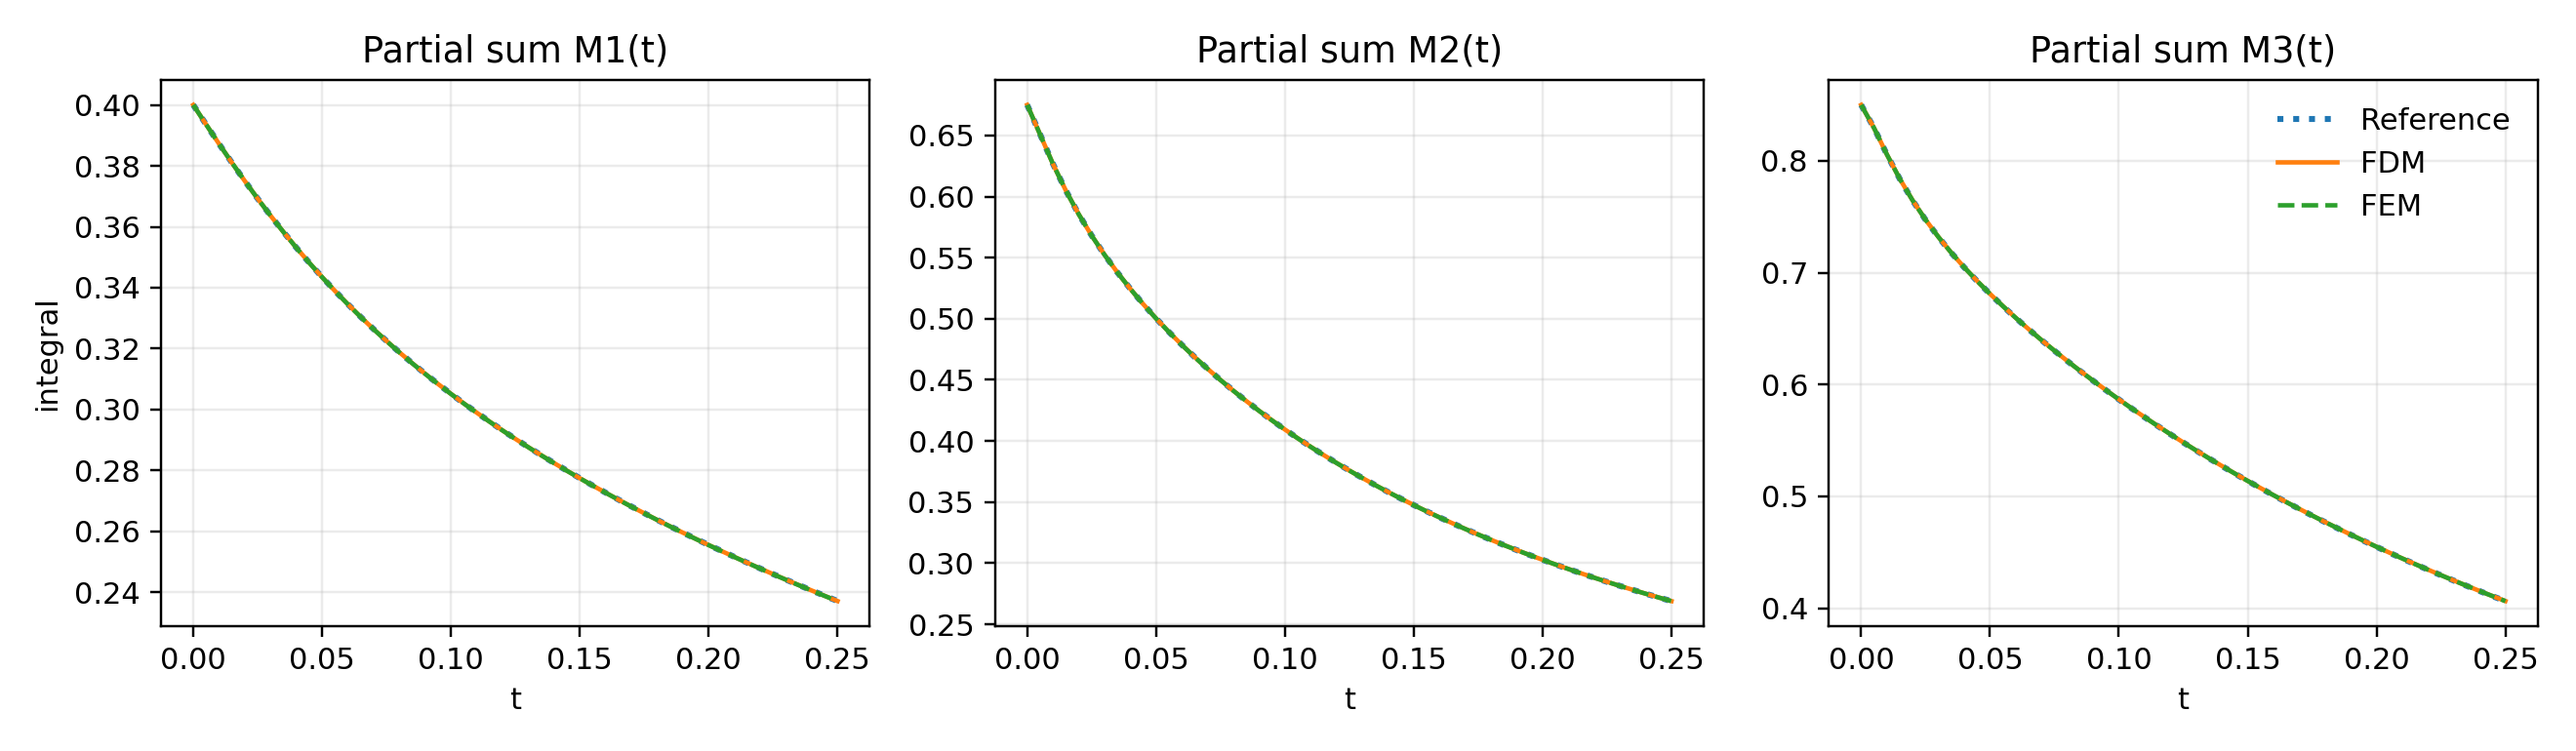
\includegraphics[width=.96\textwidth]{figures/three_component_partial_sums.png}
\caption{Partial-mass trajectories for the three-component benchmark. The reference, FDM, and FEM trajectories are nearly superposed on this scale; no positive time increment is detected on the evaluation grid.}
\label{fig:three-partial-sums}
\end{figure}

These results are not used as a proof of Proposition~\ref{prop:partial-sum}. Their role is narrower and directly auditable: the non-monotone diffusion vector realizes simultaneous cross terms, the preceding-gradient hypotheses are verified by separate component energy identities, and the numerical approximations reproduce the associated dissipative partial-sum behaviour. To connect the computation more directly with the stated estimate, we also evaluate the post-processed coercivity-bound consistency diagnostic below.

For $k>0$, define the computed left-hand quantity
\[
 \mathcal C_k(T)=\frac{d_3}{2}\int_0^T\!\!\int_0^1 |\partial_xT_k(U_3)|^2\,dx\,dt
\]
and the analytical upper-bound quantity
\[
 \mathcal B_k=\int_0^1\Phi_k(U_3(0,x))\,dx+\frac7{30}C_1+\frac7{12}C_2.
\]
The gradients are evaluated on the common grid and both integrals use trapezoidal quadrature. Table~\ref{tab:coercivity-diagnostic} reports the result for four truncation levels. The ratio remains below $0.221$ for the reference, FDM, and FEM fields. This is a post-processed numerical illustration of the conditional estimate, not a proof of the continuous proposition or of a discrete energy inequality.

\begin{table}[!htbp]
\centering
\caption{Post-processed coercivity-bound consistency diagnostic for the three-component benchmark.}
\label{tab:coercivity-diagnostic}
\begin{tabular}{lcccc}
\toprule
Method & $k$ & $\mathcal C_k(T)$ & $\mathcal B_k$ & $\mathcal C_k/\mathcal B_k$\\
\midrule
Reference & $0.25$ & $0.04650$ & $0.50479$ & $0.0921$\\
Reference & $0.50$ & $0.09450$ & $0.63395$ & $0.1491$\\
Reference & $1.00$ & $0.15815$ & $0.74661$ & $0.2118$\\
Reference & $2.00$ & $0.16484$ & $0.74917$ & $0.2200$\\
FDM & $1.00$ & $0.15822$ & $0.74661$ & $0.2119$\\
FEM & $1.00$ & $0.15819$ & $0.74661$ & $0.2119$\\
\bottomrule
\end{tabular}
\end{table}


\subsection{Independent residual, initial-data mismatch, and training variability}

The PINN RMSE values for seeds 11, 29, 47, 71, and 101 are $2.710\times10^{-3}$, $3.215\times10^{-3}$, $3.663\times10^{-3}$, $3.151\times10^{-3}$, and $4.130\times10^{-3}$, respectively. Their mean and sample standard deviation are $(3.374\pm0.541)\times10^{-3}$. On the same 5000 independently sampled points for every run, the root-mean-square differential residual is $0.179\pm0.097$, compared with a training-point RMS residual of $0.0525\pm0.0119$. Reporting both quantities avoids comparing a mean-square training loss directly with a root-mean-square test diagnostic.

Because the output ansatz does not impose the initial condition exactly, we also evaluate $E_{\mathrm{IC}}$ from the archived fields rather than inferring it from the loss weight. For seeds 11, 29, 47, 71, and 101 the relative initial-data errors are $4.024\%$, $3.960\%$, $4.816\%$, $3.972\%$, and $4.445\%$, respectively, with mean and sample standard deviation $4.243\%\pm0.378\%$. The corresponding initial combined RMSE is $(1.775\pm0.158)\times10^{-2}$. Thus part of the early-time PINN discrepancy is already present at $t=0$; the independent differential residual remains necessary to distinguish this initial-data mismatch from the quality of the learned PDE dynamics. The values are generated from the archived solution arrays by the supplementary script \texttt{initial\_condition\_diagnostic.py}.

\begin{figure}[!htbp]
\centering
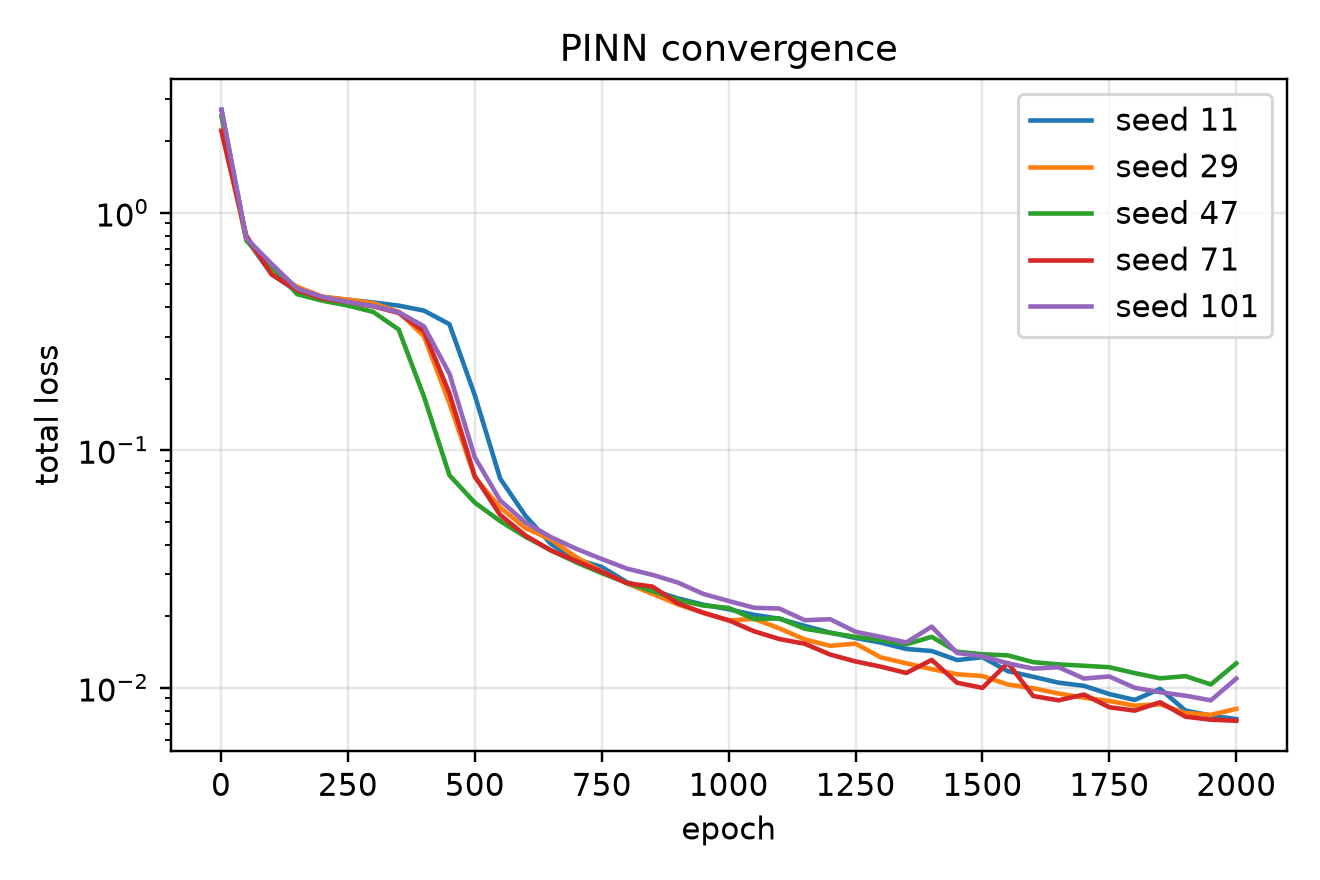
\includegraphics[width=.72\textwidth]{figures/reproducible_loss_convergence.png}
\caption{Total PINN loss for five independent seeds.}
\label{fig:computed-loss}
\end{figure}

All five loss histories decrease by more than two orders of magnitude and reach final total losses between $7.25\times10^{-3}$ and $1.26\times10^{-2}$, showing consistent loss reduction across the tested initializations. The field errors nevertheless vary by about $16\%$ relative to their mean. The common-point test residual is, on average, about $3.4$ times the training-point RMS residual, with substantial seed-to-seed variation. This gap indicates incomplete residual generalization for the tested configuration; it is not a confidence statement about the wider population of PINN trainings. Such a gap is consistent with the broader observation that PINN training objectives may be poorly balanced or may converge at different rates across loss components~\cite{wang2021gradient,wang2022ntk,krishnapriyan2021failure}.
\subsection{Collocation-size ablation}

Table~\ref{tab:ablation} fixes the architecture, seed, and $1200$-epoch budget while varying $N_f$. For seed 11, increasing the collocation set reduces the independent residual, but does not reduce RMSE at a fixed optimization budget. This single-seed ablation is a sensitivity check rather than a population-level conclusion.

\begin{table}[!htbp]
\centering
\caption{PINN collocation ablation (seed 11, 1200 epochs).}
\label{tab:ablation}
\begin{tabular}{rccc}
\toprule
$N_f$ & RMSE & Independent residual & Training time (s)\\
\midrule
1000 & $4.230\times10^{-3}$ & $0.371$ & $25.0$\\
3000 & $4.806\times10^{-3}$ & $0.151$ & $51.7$\\
6000 & $5.116\times10^{-3}$ & $0.103$ & $95.0$\\
\bottomrule
\end{tabular}
\end{table}

The ablation separates sampling coverage from optimization quality. Sampling density and residual-point placement are known to interact strongly with PINN accuracy, motivating adaptive strategies in more demanding settings~\cite{wu2023sampling}. Raising $N_f$ from $1000$ to $6000$ lowers the independent residual from $0.371$ to $0.103$, a reduction of about $72\%$, but raises the field RMSE from $4.23\times10^{-3}$ to $5.12\times10^{-3}$ and increases training time by a factor of about $3.8$. With the number of epochs fixed, the larger collocation problem receives less optimization effort per residual condition. For this seed, the result supports joint tuning of sampling density and training budget; it does not imply that additional collocation points are intrinsically detrimental or that the trend is robust across initializations.

\subsection{Positivity and mass-control diagnostic}

FDM and FEM remain nonnegative up to floating-point roundoff on the evaluation grid; their reported minimum $8.25\times10^{-33}$ represents a theoretical zero in the initial data. The PINN interior minimum is $(5.786\pm0.051)\times10^{-3}$ because the softplus representation is strictly positive away from the boundary. No positive time increment of the trapezoidal total mass is observed. For the PINN, non-negativity and boundary values are exact consequences of the output transformation; mass monotonicity remains an a posteriori observation.

\begin{figure}[!htbp]
\centering
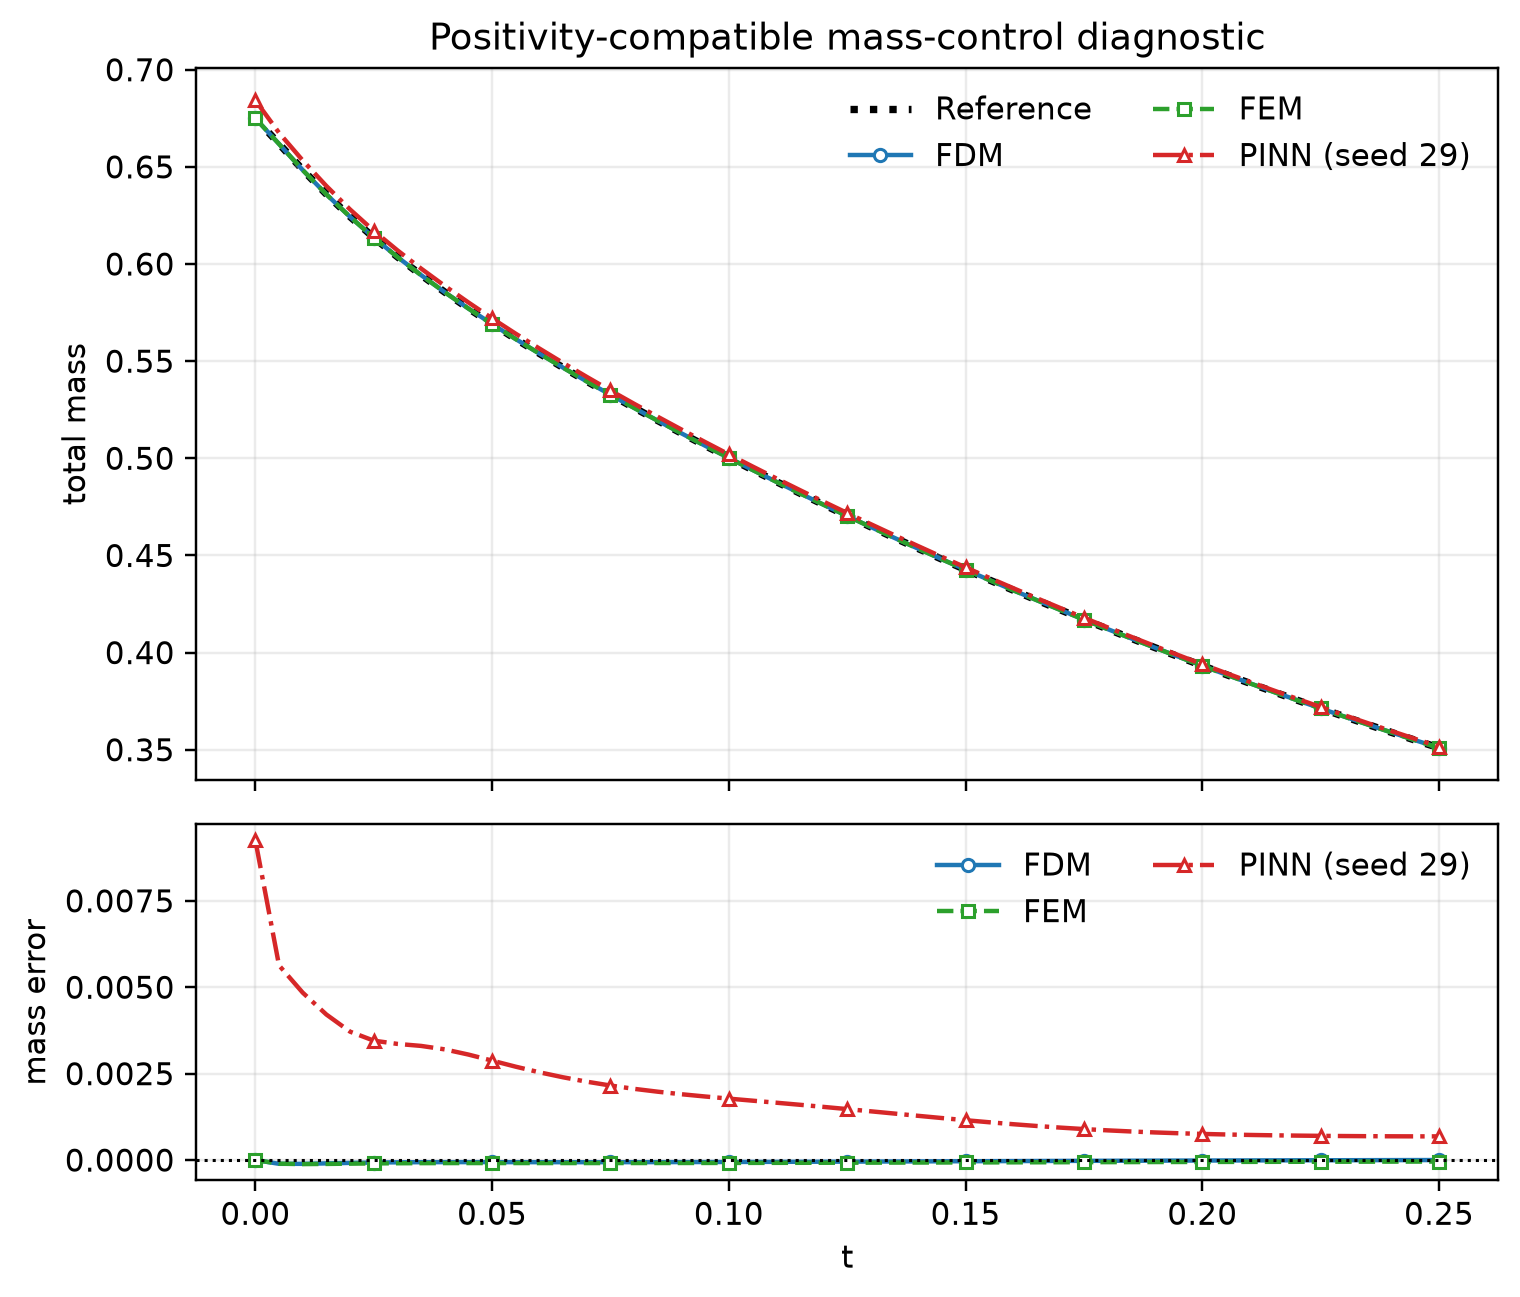
\includegraphics[width=.72\textwidth]{figures/reproducible_mass_control.png}
\caption{Mass-control diagnostic. Top: total-mass trajectories, distinguished by line style and spaced markers; the reference, FDM, and FEM curves nearly coincide. Bottom: signed mass error relative to the reference, which resolves the otherwise hidden differences. Under Dirichlet conditions, boundary fluxes also enter the mass balance. Positivity is assessed separately through the reported interior minima.}
\label{fig:computed-mass}
\end{figure}

The reference total mass decreases monotonically from $0.675$ to $0.351$, a reduction of approximately $48\%$. FDM and FEM reproduce the terminal value to within about $1.1\times10^{-6}$ and $4.3\times10^{-5}$, respectively. The median-RMSE PINN (seed 29) follows the same decreasing trend, although its initial mass is $0.684$ rather than $0.675$ because the initial condition is imposed by a penalty rather than exactly by the output ansatz. Consequently, the observed PINN mass monotonicity is encouraging but is not a discrete conservation theorem. For homogeneous Dirichlet data, the decay also combines the nonlinear sink with outward boundary flux and cannot be attributed to the reaction term alone.

\subsection{Energy-identity diagnostic}

Equation~\eqref{eq:u-energy} supplies a direct link between the analytical hypothesis and the computations. On the common grid, we evaluate
\begin{align*}
 \mathcal D_A(t)&=E_{u,A}(t)-E_{u,A}(0)
 +\int_0^t\!\left[d_1\|\partial_xu_A(s)\|_{L^2}^2
 +\int_0^1u_A^2|\partial_xu_A|^2\,dx\right]ds,\\
 E_{u,A}(t)&=\frac12\|u_A(t)\|_{L^2}^2.
\end{align*}
using centred spatial differences and trapezoidal quadrature for every archived field. This post-processed defect tests consistency with the continuous identity; it is not an exact discrete energy law of the algorithms.

\begin{figure}[!htbp]
\centering
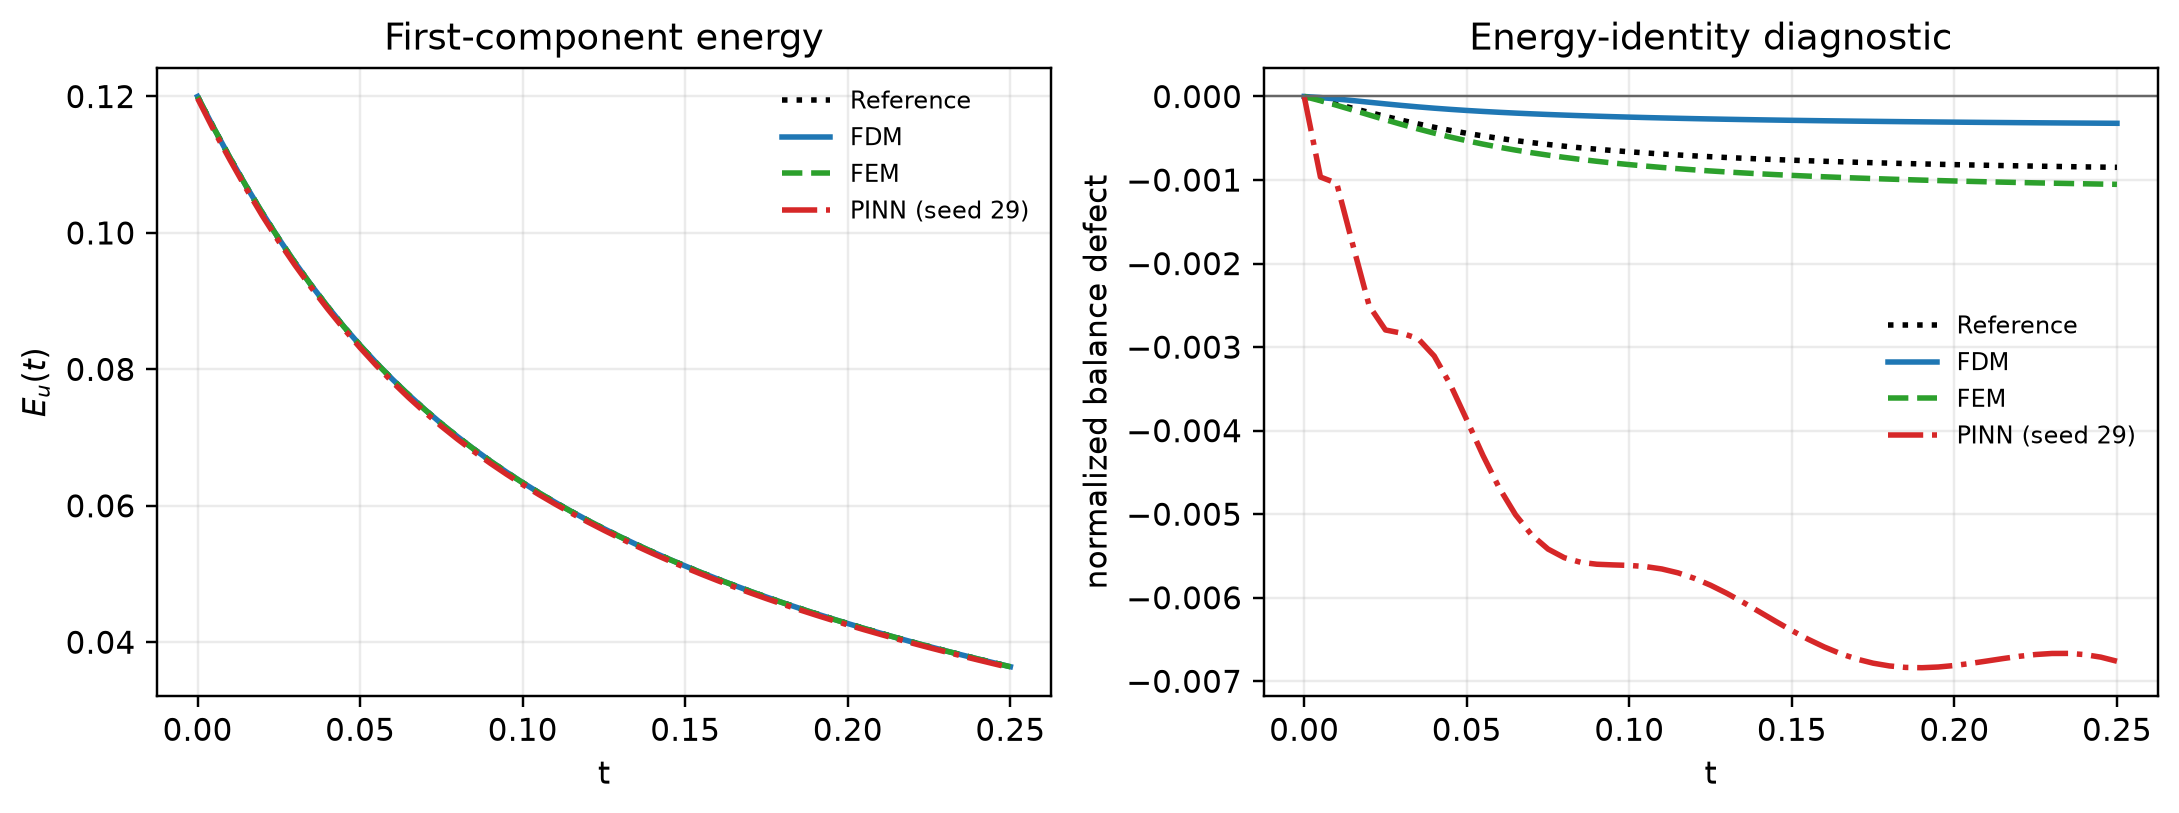
\includegraphics[width=.9\textwidth]{figures/reproducible_energy_diagnostic.png}
\caption{First-component energy and normalized defect in the continuous balance~\eqref{eq:u-energy}, evaluated on the common grid. The PINN curve is seed 29, the median-RMSE realization.}
\label{fig:energy-diagnostic}
\end{figure}

The maximum normalized defects are $8.48\times10^{-4}$ for the refined reference, $3.21\times10^{-4}$ for FDM, $1.05\times10^{-3}$ for FEM, and $6.84\times10^{-3}$ for the seed-29 PINN. All fields reproduce the decreasing first-component energy. The larger PINN defect is consistent with its larger derivative-sensitive residual, whereas the nonzero reference defect quantifies the effect of sampling and post-processing quadrature. Because the diagnostic is evaluated after interpolation to the common grid, it should not be used to infer a formal discrete energy order.
\subsection{Cross-validation of numerical claims}

Figure~\ref{fig:validation-diagnostics} assembles three diagnostics that answer different validation questions. Reference refinement checks that the comparison target is substantially more accurate than the reported methods. The collocation plot separates strong-form residual reduction from field accuracy. The error--runtime plot shows the implementation-dependent cost of constructing each representation. These panels should be read together; none alone constitutes a general ranking of the methods.

\begin{figure}[!htbp]
\centering
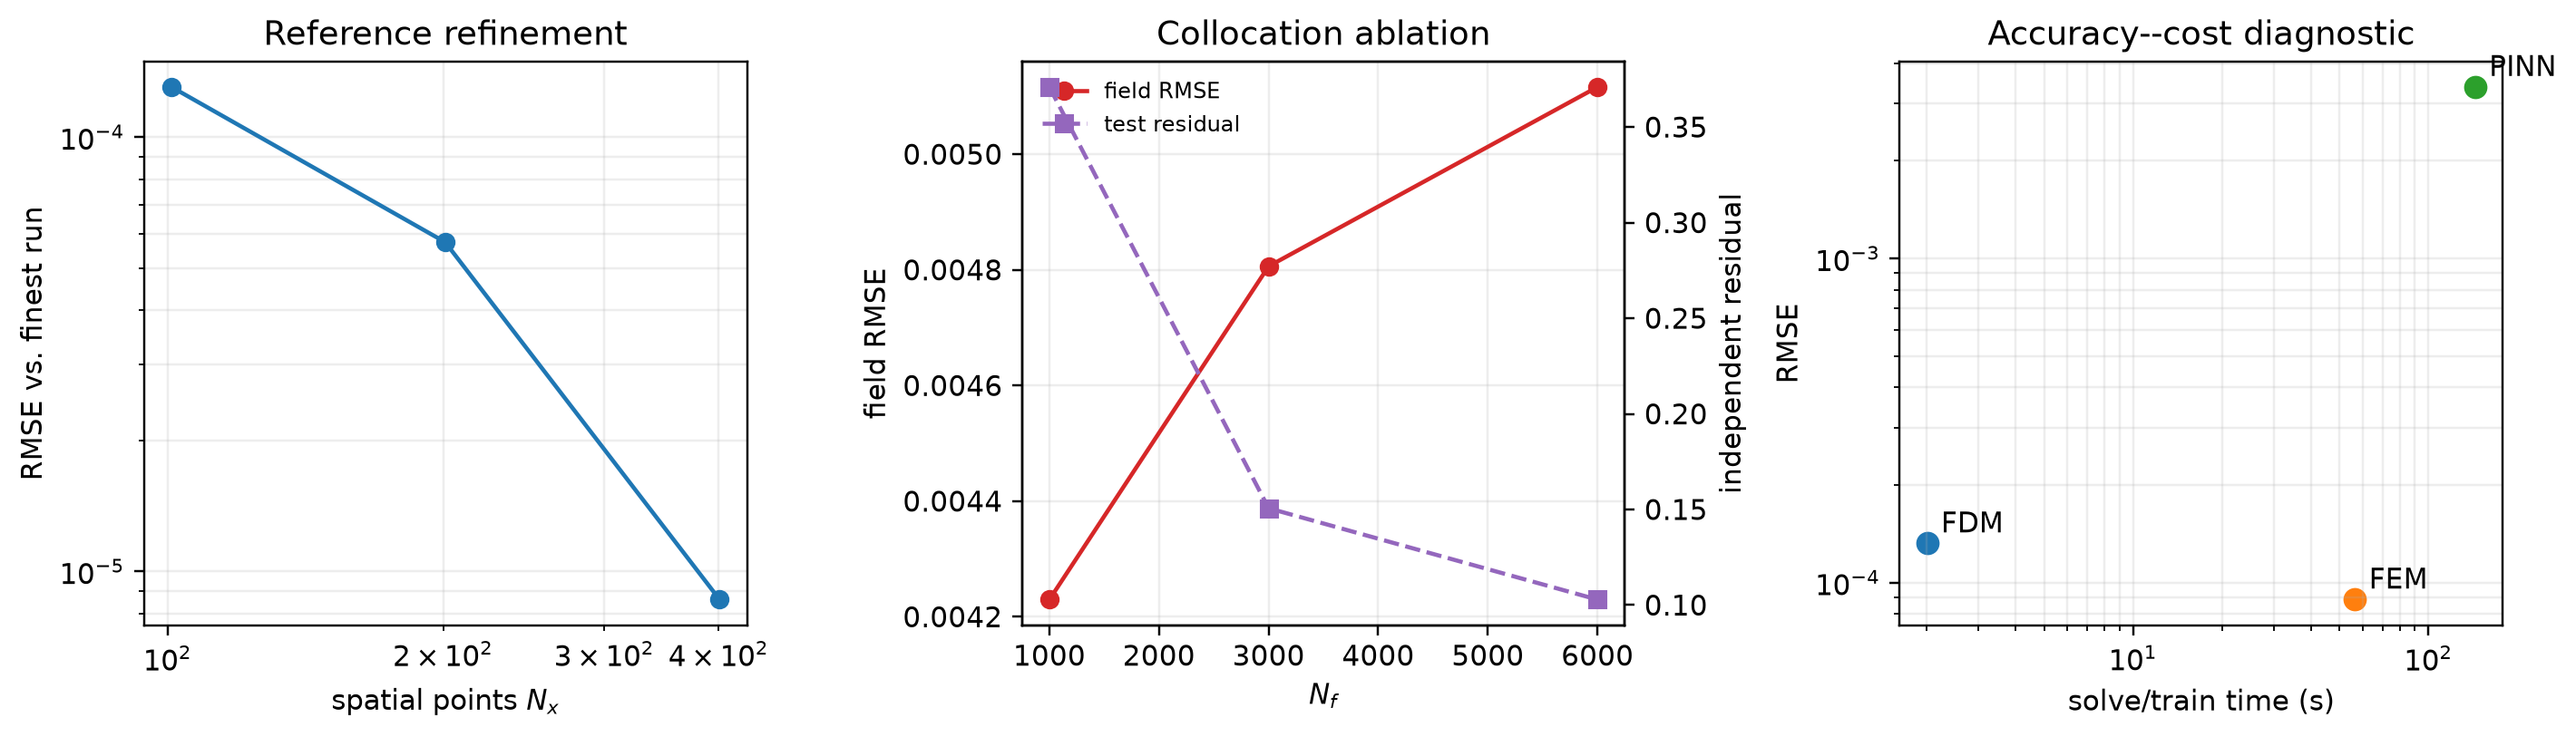
\includegraphics[width=\textwidth]{figures/reproducible_validation_diagnostics.png}
\caption{Reference-refinement, PINN collocation, and accuracy--cost diagnostics generated from the archived CSV outputs. The finest reference run has zero self-error and is therefore omitted from the logarithmic refinement curve.}
\label{fig:validation-diagnostics}
\end{figure}

The left panel verifies that refinement moves the reference solution toward the finest computation: the RMSE falls from $1.30\times10^{-4}$ at $N_x=101$ to $8.62\times10^{-6}$ at $N_x=401$. Because space and time are refined simultaneously and not at a uniform ratio, this curve is a consistency check rather than an estimate of a formal convergence order. The middle panel makes visible the residual--field-error mismatch discussed above. The right panel places the three reported implementations on distinct implementation-level accuracy--runtime regimes. For this forward 1D problem the classical solvers dominate the reported construction time and accuracy, whereas the possible advantage of the PINN lies in its differentiable continuous representation and inexpensive repeated evaluation after training. These timings are not hardware-normalized complexity measurements. A fair assessment of repeated-evaluation advantage would require many-query, inverse, or parametric experiments.

\subsection{Limitations}

The experiments concern smooth one-dimensional forward problems over short time intervals, including one two-component and one three-component non-monotone benchmark. They do not establish an error estimate for PINNs and do not address inverse problems or high-dimensional geometry. The PINN study is a controlled diagnostic rather than a state-of-the-art optimization contest: FDM/FEM use float64, whereas the reported PINN uses float32, Adam only, one architecture, and a fixed initial-condition weight; the resulting initial-data error is therefore reported explicitly rather than hidden inside the training loss. The common unforced reference is generated by refined FDM, which can in principle favor the same discretization family; the separate MMS verification, the 401-versus-801 refinement check, and the fact that the reported FEM error is lower than the coarse-FDM error reduce but do not eliminate this dependence. Runtime comparisons are implementation-specific, and Python allocation tracking omits native-library allocations. FP64 Adam--L-BFGS, loss-weight sensitivity, causal training, and higher-dimensional tests are therefore natural extensions rather than claims of the present study.

\section{Conclusion and perspectives}
\label{sec:conclusion}

We have derived an exact partial-sum calculation for triangular reaction--diffusion systems with critical gradient growth. The exact tested identity contains the full gradients of preceding components. If these gradients are uniformly bounded in $L^2(Q_T)$, Young's inequality with a free parameter absorbs all cross terms for any fixed positive diffusion vector; no diffusion ordering is intrinsic to this conditional step. Conversely, bounds on $\nabla T_k(u_{j,n})$ alone do not justify the same conclusion. The main analytical contribution is the identification of this exact full-gradient cross-term structure and the resulting conditional coercivity estimate for any fixed positive diffusion vector. An important consequence is the explicit separation between the algebraic absorption step and the compactness theory that must still be supplied by the chosen solution framework.

The numerical contribution now has three complementary levels. First, an independent manufactured-solution experiment verifies the implementations of the classical solvers: spatial refinement gives approximately second-order RMSE behaviour for both FDM and the assembled $P_1$ FEM, while separate temporal refinement gives first-order behaviour for the semi-implicit update. Second, the two-component benchmark retains the reproducible PINN--FDM--FEM comparison, common-point independent residual testing, five-seed descriptive statistics, an explicit $4.243\%\pm0.378\%$ relative initial-data mismatch, mass and energy diagnostics, and collocation ablation. On that smooth forward problem, the classical methods remain substantially more accurate and cheaper to construct than the PINN, while the PINN provides a nonnegative boundary-compatible differentiable surrogate. Third, the new three-component benchmark uses the non-monotone diffusion vector $(0.1,0.8,0.3)$ and realizes two simultaneous cross terms in a controlled structural test. The preceding-gradient bounds are established independently as $C_1\le1.2$ and $C_2\le0.0708984375$, yielding a residual Young contribution bounded by $0.321357421875$. A post-processed coercivity-bound consistency diagnostic over four truncation levels gives $\mathcal C_k/\mathcal B_k<0.221$ for the refined reference and essentially the same ratios for FDM and FEM. Against the refined numerical reference, the three-component FDM and FEM attain RMSE values $1.48\times10^{-4}$ and $1.14\times10^{-4}$, respectively, while remaining nonnegative and exhibiting non-increasing partial masses on the common evaluation grid.

The scope is therefore precise. Proposition~\ref{prop:partial-sum} is a conditional coercivity result whose full-gradient hypothesis must come from the surrounding analytical framework; the three-component experiment provides a controlled one-dimensional realization of that structure. The numerical comparison is correspondingly diagnostic: it separates field error, residual generalization, initial-data mismatch, and structural observables on the tested forward problem. Extension to a complete existence theorem, higher-dimensional or inverse settings, or a calibrated application requires the additional analytical and modelling ingredients identified below.

\subsection*{Perspectives}

Three directions follow naturally. On the analytical side, the priority is to derive the full preceding-gradient estimates from independently checkable hypotheses, or to replace them by a duality, entropy, or renormalized argument that closes the compactness proof. Weighted lower-triangular structures, no-flux boundary conditions, uniqueness, and long-time behaviour are further relevant extensions. On the numerical side, FP64 Adam--L-BFGS, loss-balancing strategies motivated by known gradient-flow pathologies~\cite{wang2021gradient,wang2022ntk}, causality-aware training~\cite{wang2024causality}, and adaptive residual sampling~\cite{wu2023sampling} should be compared under matched computational budgets; two-dimensional domains, stiff diffusion contrasts, inverse identification, and residual-based a posteriori indicators would test whether the differentiable surrogate offers a genuine advantage. On the modelling side, the transfer--dissipation chain can be specialized to a selected interfacial chemical, biological, materials, or image-processing problem only after dimensional consistency and measurable observables have been specified. These extensions would turn the present auditable benchmark into either a complete analytical theorem or a validated application study.

\subsection*{Code and data availability}
The supplementary reproducibility archive contains the code, fixed configurations and seeds, raw metrics, solution arrays, independent-residual, initial-condition and ablation outputs, refinement data, dependency specification, and figure-generation routines used for the reported results. The archived scripts regenerate the validation figures and post-processed diagnostics from the stored outputs without requiring the solvers to be rerun.

\subsection*{Acknowledgments}
The authors acknowledge the computational resources provided by the National School of Applied Sciences of Safi, Cadi Ayyad University, Morocco.

% -----------------------------------------------------------------------------
% Statements and Declarations
% MJM requires relevant declarations at submission. Fill these from verified
% author information; do not submit placeholders as factual statements.
% -----------------------------------------------------------------------------
% Uncomment the block below only after all authors have verified the statements.
% \section*{Statements and Declarations}
% \textbf{Competing Interests.} [Insert verified declaration.]
% \textbf{Funding.} [Insert verified funding statement.]
%
% Springer Nature's current journal instructions state that non-copy-editing use
% of an LLM/AI tool should be documented in the Methods section or another
% suitable part of the manuscript. Insert an accurate, human-approved disclosure
% if applicable to the final submitted work.
% \textbf{Use of AI-assisted tools.} [Insert accurate disclosure if required.]

% -----------------------------------------------------------------------------
% References
% birkjour is AMSart-based; amsplain gives a conventional numbered mathematics
% bibliography. Keep bibliography.bib in the same submission directory.
% -----------------------------------------------------------------------------
\bibliographystyle{amsplain}
\bibliography{bibliography}

\end{document}
